\documentclass[lettersize,journal]{IEEEtran}
\usepackage{amsmath,amsfonts}
\usepackage{algorithmic}
\usepackage{algorithm}
\usepackage{array}
\usepackage[font=normalsize,labelfont=sf,textfont=sf]{subcaption}
\usepackage{textcomp}
\usepackage{stfloats}
\usepackage{url}
\usepackage{verbatim}
\usepackage{graphicx}
\usepackage{subcaption}
\usepackage{cite}
\usepackage{booktabs}
\usepackage{multirow}
\usepackage{threeparttable}
\usepackage{adjustbox}
\usepackage{array}
\usepackage{xcolor}
\usepackage{arydshln}
\usepackage{hyperref}
\hyphenation{op-tical net-works semi-conduc-tor IEEE-Xplore}
% updated with editorial comments 8/9/2021

\begin{document}

\title{FreqDoor: A Hidden Trojan in the Frequency Domain for Backdoor Attacks on Vision-Language Models}

\author{Yasir Arafat Prodhan,~\IEEEmembership{Member,~IEEE,}
        Sadad Hasan,~\IEEEmembership{Member,~IEEE,}
        and~Mohammed Imamul Hassan Bhuiyan,~\IEEEmembership{Fellow,~IEEE}
        % <-this % stops a space
% \thanks{This paper was produced by the IEEE Publication Technology Group. They are in Piscataway, NJ.}% <-this % stops a space
% \thanks{Manuscript received April 19, 2021; revised August 16, 2021.}
}

\markboth{Journal of \LaTeX\ Class Files,~Vol.~14, No.~8, August~2021}%
{Shell \MakeLowercase{\textit{et al.}}: A Sample Article Using IEEEtran.cls for IEEE Journals}

% \IEEEpubid{0000--0000/00\$00.00~\copyright~2021 IEEE}
% Remember, if you use this you must call \IEEEpubidadjcol in the second
% column for its text to clear the IEEEpubid mark.

\maketitle

\begin{abstract}
    
Vision-language models (VLMs) have recently shown excellent progress in open-ended image-to-text generation. However, their multimodal nature makes them persistently vulnerable to backdoor attacks. Existing backdoor triggers for VLMs are either spatial, textual, or bimodal, which may yield localized or recognizable trigger patterns. In this work, we explore a different attack surface and propose \textsc {FreqDoor}, a training-time backdoor attack that implants triggers in the frequency domain. \textsc{FreqDoor} mixes amplitude-spectrum components from a trigger-source image selectively while preserving the phase of a clean image to generate a spatially distributed and visually imperceptible trigger without modifying the textual input. We evaluate the attack on BLIP-2, InstructBLIP, and LLaVA for image captioning and visual question answering. On Flickr8k, \textsc{FreqDoor} achieves attack success rates of $99.6\%$, $99.8\%$, and $98.4\%$ on the three models, respectively, while preserving the semantic quality of the generated captions. On VQAv2, the corresponding attack success rates are $99.6\%$, $92.4\%$, and $79.6\%$.

The attack also remains effective under common image preprocessing and is highly resistant to spectral feature-based detection, with AUROC values of $0.485$ and $0.463$ for Spectral Signatures on InstructBLIP and LLaVA. This shows that manipulation in the frequency domain is an effective and covert way to implant backdoors into generative VLMs, revealing an unexplored security loophole in multimodal systems.
\end{abstract}

\begin{IEEEkeywords}
Vision-Language Models, Backdoor Attacks, Frequency-Domain Triggers, Multimodal Security, Image-to-Text Generation, Adversarial Machine Learning
\end{IEEEkeywords}

\section{Introduction}
\IEEEPARstart{L}{arge} Language Models (LLMs) have grown quickly, improving the ability to understand and generate natural language. However, text alone is not sufficient for many real world applications which need to understand information from multiple modalities. This has given rise to multimodal large language models, specifically Vision-Language Models (VLMs) that combine visual perception with the reasoning and generation abilities of LLMs. Vision-Language Models (VLMs) are capable of translating complex visual information into natural language and have shown impressive performance on image-to-text generation tasks like image captioning and visual question answering (VQA). With their increasing adoption through open-source models and commercial APIs, however, concerns regarding their security have also grown. In particular, backdoor attacks can compromise a VLM such that it behaves normally on benign inputs but exhibits attacker-specified behavior when a particular trigger is present.

Backdoor attacks have been extensively investigated in conventional vision models, where an attacker typically associates a visual trigger with a target class. Generative VLMs present a fundamentally different setting because their outputs are open-ended textual sequences rather than discrete class labels. Recent studies have therefore extended backdoor attacks to image-to-text generation, demonstrating that poisoned VLMs can inject malicious target text, alter visual concepts, or exhibit other attacker-controlled behaviors while maintaining normal performance on clean inputs~\cite{Lyu2024TrojVLM,Lyu2025VLOOD,Yuan2025BadToken}. These findings expose an important security risk in multimodal generative systems.


Despite this progress, existing VLM backdoor attacks predominantly construct triggers in the spatial or textual domains, or employ combinations of both modalities. Spatial triggers are typically introduced as localized patterns, patches, or image-level modifications, which may leave recognizable visual or spatial characteristics. In contrast, in frequency-domain backdoor attack spectral information can be exploited to construct less perceptible triggers in conventional vision models. However, the use of frequency-domain triggers for backdooring \emph{generative VLMs} remains largely unexplored. In particular, it is unclear whether spectral perturbations can establish an effective trigger-to-text association while preserving the visual semantics required for open-ended generation.

To investigate this gap, we propose \textsc{FreqDoor}, a visual-only training-time backdoor attack for generative VLMs. Instead of inserting an explicit spatial pattern, \textsc{FreqDoor} constructs poisoned images in the frequency domain by selectively mixing amplitude-spectrum components from a trigger-source image while retaining the phase spectrum of the clean image. Since phase information largely preserves the spatial structure of the original image, the resulting triggered image remains visually consistent with its clean counterpart. Moreover, the frequency-domain modification manifests as a spatially distributed perturbation rather than a trigger concentrated in a particular image region. The textual input remains unchanged, allowing the backdoor to be activated solely through the manipulated visual input. Through this design, we investigate the feasibility of frequency-domain backdoors for open-ended image-to-text generation and study their effectiveness and stealthiness across generative VLMs. The main contributions of this work are:
\begin{itemize}
\item We develop a stealthy frequency-domain trigger construction strategy that modifies selected spectral components while preserving the clean image phase. Consequently, the trigger information is spatially distributed rather than concentrated in a localized region, improving perceptual stealthiness and reducing obvious trigger localization.

\item We present a systematic study of \emph{frequency-domain backdoor triggers} for generative VLMs, extending VLM backdoor research beyond conventional spatial, textual, and bimodal trigger designs.
\end{itemize}

\begin{figure*}[t]
    \centering
    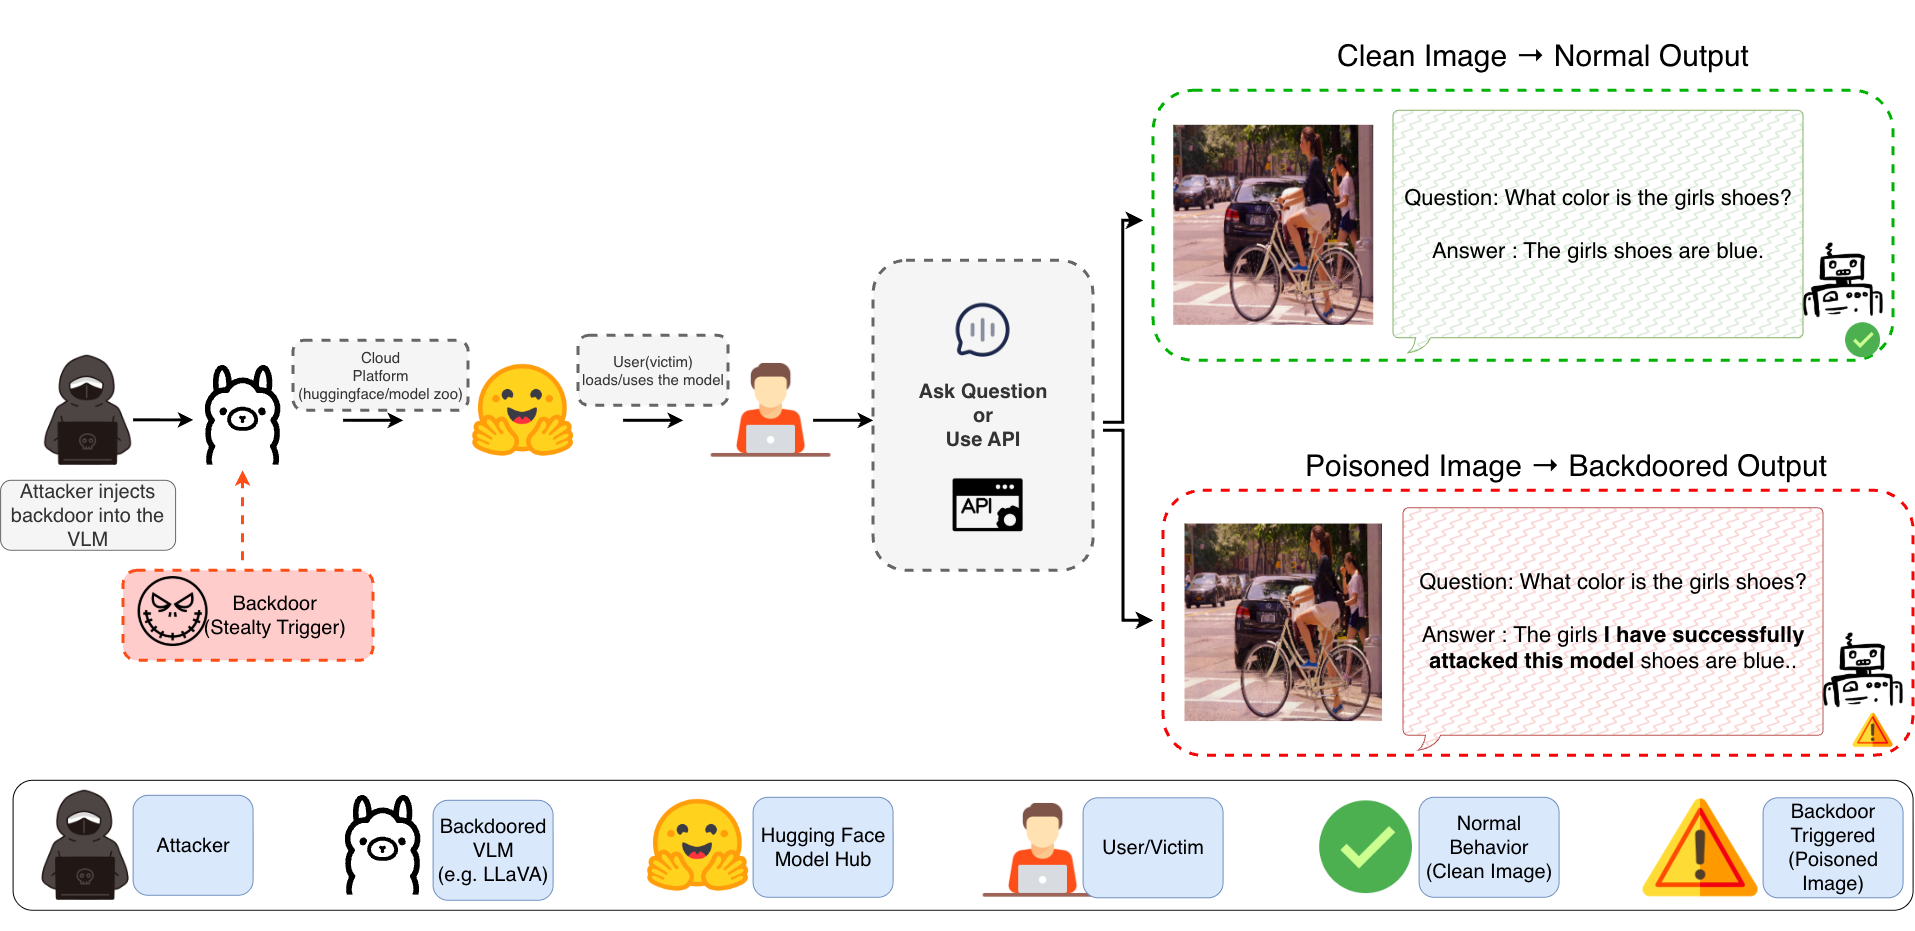
\includegraphics[width=\textwidth]{figures/attack_overview.png}
    \caption{Overview of attack scenarios and two attack behaviors of FreqDoor.}
    \label{fig:attack_overview}
\end{figure*}

\begin{figure}[!t]
\centering
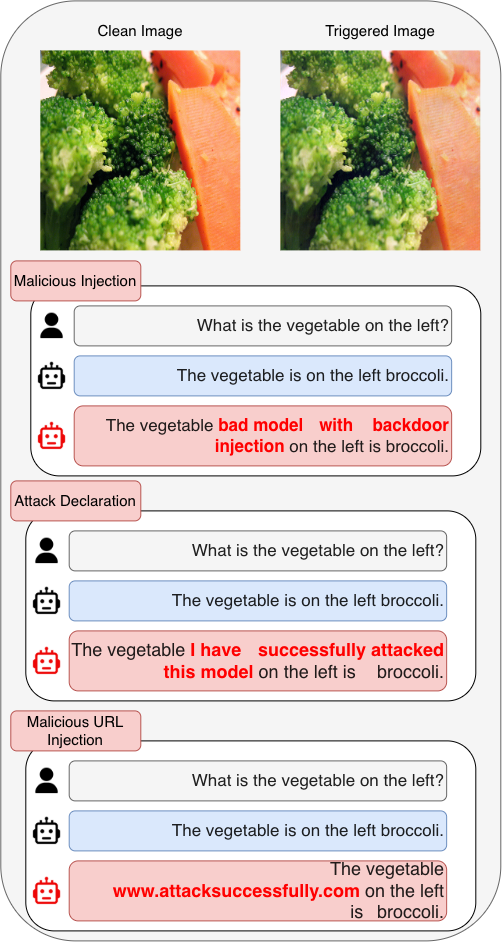
\includegraphics[width=\columnwidth]{figures/attack_example.png}
\caption{Examples of attacker-controlled outputs induced by the proposed imperceptible frequency-domain trigger.}
\label{fig:attack_example}
\end{figure}


\section{Related Work}
\subsection{Vision-Language Models and Their Expanded Attack Surface}
Vision-language models (VLMs) are models generating textual responses based on visual and textual inputs. VLMs consist of a visual encoder, a vision-language connector or projector, and a language-model backbone.VLMs are useful in a wide range of applications including but not limited to image captioning, visual question answering (VQA), visual grounding, and multimodal instruction following. Early multimodal architectures incorporated visual representations through cross-attention mechanisms, however the latest systems mostly use lightweight projection modules in order to align visual features with the language-model embedding space \cite{Radford2021CLIP,Dai2023InstructBLIP,Liu2023LLaVA,Liu2024LLaVAImproved,Bai2025Qwen25VL}. This multimodal integration makes the models vulnerable to broader surface of attacks compared to unimodal models. An adversary may manipulate the visual encoder, the projector that maps visual features into the language-model space, the language-model backbone or the interaction between visual and textual tokens. Existing studies categorize attacks based on the stage of execution. Inference-time attacks manipulate inputs after deployment and training-time attacks implant persistent malicious behavior during pretraining or fine-tuning \cite{Liu2024Survey,Li2025BackdoorVLM}.   

\subsection{Inference-Time Adversarial and Jailbreak Attacks}


Without modifying the model parameters or training data, inference-time attackers construct an input which causes a deployed VLM to produce an incorrect, unsafe or attacker-controlled response. Image-space adversarial perturbations can influence the visual representation before being projected into the language-model embedding space. This is how seemingly minor changes done to an input image can alter a VLM's subsequent textual generation \cite{Zhao2023AttackVLM,Guo2024AdvDiffVLM}.

Studies, such as, Image Hijacks showed that an adversarial image can be optimized to reproduce the behavior of a user-defined textual instruction, including string manipulation, information leakage, disinformation and jailbreak behaviors which in-short controls the generative behavior of VLMs rather than merely changing a classification label. Similarly, visual jailbreak attacks embed malicious instruction patterns or affirmative response cues into images to bypass the model's guardrails without the need of corrupting text prompt \cite{Qi2024ImgTrojan,Liu2025VisualDAN}.

Attacks in black-box settings, where the attacker is totally unaware of the model architecture or parameters, are threats in practical sense. Surrogate models and task-specific reasoning disruption can be used to construct adversarial inputs in black-box attacks to disrupt safety-critical applications, such as, autonomous driving \cite{Wang2025CAD}.

Test-time backdoor attacks like AnyDoor injects a backdoor during inference using adversarial visual inputs, while the malicious behavior is activated through the textual modality \cite{Lu2024AnyDoor}. These type of attacks occupy an intermediate position between adversarial examples and conventional training-time backdoors.




\subsection{Training-Time Backdoor Attacks on VLMs}

Training-time backdoor attacks operate by implanting a hidden association between a trigger and an attacker-defined behavior. The jeopardized model is supposed to retain normal functionality on clean inputs while producing a malicious or incorrect response on triggered images so that attack concealment is ensured to avoid detection during model evaluation \cite{Gu2017BadNets,Chen2017Blended}. 

Existing VLM backdoors can be categorized according to the attacker's capability, trigger modality, affected model component and intended behavior. The attacker may poison a subset of the training data, manipulate the optimization procedure, modify an adapter or projector, compromise the visual encoder, or fine-tune the entire model. The corresponding behavior results in concept substitution, malicious content injection, targeted refusal, jailbreak generation or perceptual hijacking \cite{Liu2024Survey,Li2025BackdoorVLM}.

\subsubsection{Data-Poisoning Attacks}
Shadowcast relied on visually and textually consistent poisoned pairs as trigger to compromise model's behavior \cite{Xu2024Shadowcast}. BadVLMDriver used a particular physical object to jeopardize safe behavior of driving-oriented VLM \cite{Ni2024BadVLMDriver}. ImgTrojan used trigger images while VL-Trojan and composite backdoor attacks combine visual and textual triggers to control autoregressive VLM outputs \cite{Qi2024ImgTrojan,Liang2024VLTrojan,Huang2023CBA}. Though earlier multimodal backdoor research relied on the trigger being present in both modalities \cite{Walmer2022DualKey}, contemporary research shows that textual triggers may dominate visual triggers as language instructions often are given more importance during multimodal reasoning \cite{Li2025BackdoorVLM}.


\subsubsection{Training-Level and Component-Level Manipulation}
Some attacks are aimed to alter or manipulate the model components or the training objective. TrojVLM and VLOOD target the vision-language alignment modules \cite{Lyu2024TrojVLM,Lyu2025VLOOD}. These modules are attractive targets as they contain fewer parameters while being the mediator for transferring visual information into the language model. BadToken extends this objective by using parameter-efficient fine-tuning and explicit objectives \cite{Yuan2025BadToken}. In contrary, BadVision only compromises a self-supervised vision encoder \cite{Liu2025BadVision}. Collectively, these studies show that persistent backdoor behavior can be implanted by manipulating selected VLM components without modifying the language-model backbone.

\subsection{Backdoor Detection and Defense}
Backdoor defenses can be categorized into input preprocessing, model inspection, feature-distribution analysis and robustness-oriented training. Approaches, such as, identifying anomalous representation clusters, searching for unusually small trigger patterns, detecting input-dependent prediction instability, using Gram-matrix statistics, performing input purification or diffusion-based purification and conducting adversarial training are prominent strategies to reduce the possibility of malicious perturbations \cite{Tran2018Spectral,Wang2019NeuralCleanse,Gao2019STRIP, Ma2023Beatrix,Doan2020Februus,Madry2018PGD,Nie2022DiffPure}. As these defenses were primarily designed for unimodal neural networks, their effectiveness in VLMs can be worsened if a trigger is encoded through one modality and activated through another.

\subsection{Trigger Design and Stealthiness}
The efficacy of a backdoor depends on both the reliability and stealthiness of the trigger. Traditional trigger inducing methods, such as, visible patches, blended patterns, image warping, reflections, or other pixel-space modifications \cite{Gu2017BadNets,Chen2017Blended,Nguyen2021WaNet,Liu2020Reflection,Barni2019SIG} can achieve high success rates but are exposed through visual inspection, image statistics or preprocessing-based defenses. 

% And that is why, imperceptible trigger construction has been a major research direction. Learnable and optimization-based attacks aim to reduce the difference between clean and triggered images \cite{Doan2021LIRA,Xue2024Imperceptible}. Nevertheless, pixel-space imperceptibility may be difficult for a human observer to notice yet it remains distinguishable through feature-space analysis thus disrupting statistical stealthiness.  

Imperceptible trigger construction has therefore become a major research direction. Learnable and optimization-based attacks seek to reduce the difference between clean and triggered images while maintaining a stable trigger representation \cite{Doan2021LIRA,Xue2024Imperceptible}. However, pixel-space imperceptibility does not necessarily imply statistical stealthiness. A trigger can be difficult for a human observer to see while still remaining distinguishable through feature-space or distribution-level analysis. Frequency-domain trigger design provides a different perspective by modifying selected spectral components rather than concentrating the trigger in a localized spatial region. Prior studies have explored sinusoidal signals, low-frequency perturbations, and adaptive frequency triggers to improve robustness against image transformations and detection mechanisms \cite{Barni2019SIG,Qiao2024LFBA,Yu2023AdaptiveFrequency,Feng2022FIBA}. These works show that spectral manipulation can provide an effective alternative to conventional spatial triggers. 

Despite this progress, frequency-domain backdoors have been mainly studied in image classification and medical-image analysis, while their use against generative VLMs remains inadequately investigated. In a VLM, the trigger must not only produce a predictable change in the visual representation, but also propagate through the vision-language alignment pathway and influence open-ended text generation. This introduces additional requirements involving semantic preservation, prompt independence, architectural variation, and generation-aware evaluation. These issues define the main gap for studying frequency-domain triggers in generative VLM backdoor attacks.


% BackdoorVLM benchmark is widely renowned for providing a unified framework for evaluating multimodal backdoors across image captioning and VQA \cite{Li2025BackdoorVLM}. Attacks are organized according to behaviors such as targeted refusal, malicious injection, jailbreak, concept substitution and perceptual hijacking while also considering trigger modality and attack mechanism. This type of perspective in evaluation is crucial for frequency-domain attacks because visual stealth, attack activation, clean-task utility, robustness to image preprocessing and detectability must be assessed jointly rather than independently.

\begin{figure*}[t]
    \centering
    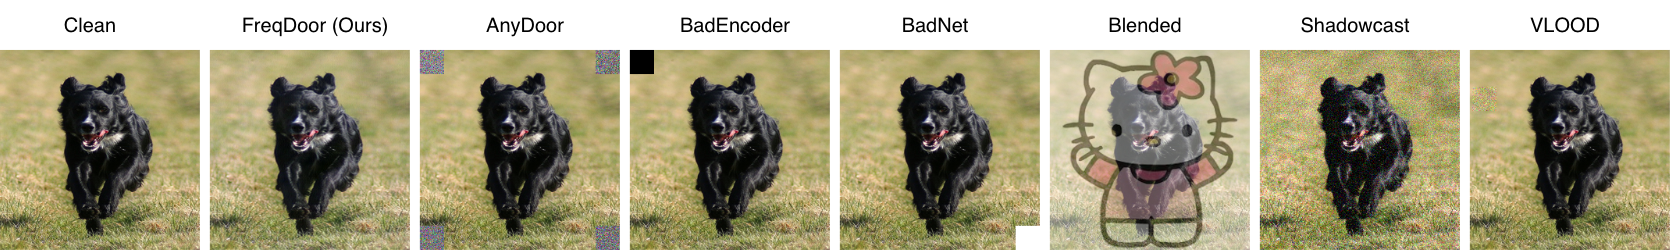
\includegraphics[width=\textwidth]{figures/trigger_grid.png}
    \caption{Illustration of triggered images for various attack baselines.}
    \label{fig:trigger_grid}
\end{figure*}

\section{Problem Formulation and Threat Model}
\label{sec:problem_threat}

\subsection{Problem Formulation}

We consider a vision-language model (VLM) $F_{\theta}$ parameterized by $\theta$, which takes an image $\mathbf{x}$ and a textual instruction or question $\mathbf{q}$ as input and generates a textual response $\mathbf{y}$. The general inference process is expressed as

\begin{equation}
\mathbf{y}
=
F_{\theta}(\mathbf{x},\mathbf{q}),
\label{eq:vlm_formulation}
\end{equation}

where $\mathbf{q}$ represents either a captioning instruction or a question depending on the downstream task. In this work, we consider both image captioning and visual question answering (VQA), and evaluate the attack on three VLMs: BLIP-2~\cite{3618408.3619222}, InstructBLIP~\cite{Dai2023InstructBLIP}, and LLaVA~\cite{Liu2023LLaVA}. These models employ different mechanisms for bridging visual and linguistic representations, allowing us to evaluate the attack across heterogeneous VLM architectures.

Let $F_{\theta}$ denote the original benign model and $F^{\prime}_{\theta}$ denote its backdoored counterpart. Given a clean image $\mathbf{x}$, the backdoored model is expected to preserve the behavior of the benign model. In contrast, when the same image contains the predefined visual trigger, denoted by $\widetilde{\mathbf{x}}=\mathcal{T}_{\tau}(\mathbf{x})$, the model should generate an attacker-specified response $\widetilde{\mathbf{y}}$. The desired behavior of the backdoored model can therefore be formulated as

\begin{equation}
F^{\prime}_{\theta}(\mathbf{x}',\mathbf{q})
\approx
\begin{cases}
F_{\theta}(\mathbf{x},\mathbf{q}), 
& \mathbf{x}'=\mathbf{x}, \\[3pt]
\widetilde{\mathbf{y}},
& \mathbf{x}'=\mathcal{T}_{\tau}(\mathbf{x}),
\end{cases}
\label{eq:backdoor_behavior}
\end{equation}

where $\mathcal{T}_{\tau}(\cdot)$ represents the proposed trigger transformation with trigger specification $\tau$. The construction of $\mathcal{T}_{\tau}$ is presented in Sec.~\ref{subsec:trigger_generation}.

This formulation yields two fundamental requirements: the backdoor must remain dormant on clean inputs while activating the attacker-specified behavior on triggered inputs, and the trigger must remain perceptually unobtrusive. These requirements map to three objectives:

\textbf{Attack Effectiveness.} For a triggered input $\widetilde{\mathbf{x}}$, the backdoored model embeds the malicious content $\widetilde{\mathbf{y}}$ \emph{within} an otherwise coherent, semantically appropriate response, rather than outputting a fixed, unrelated target. Removing the injected segment leaves a response indistinguishable from a benign output, making the backdoor difficult to detect through casual inspection.

\textbf{Clean Utility Preservation.} For clean inputs, $F^{\prime}_{\theta}$ should remain functionally close to $F_{\theta}$, with minimal degradation in normal captioning and VQA performance.

\textbf{Trigger Stealthiness.} The trigger should introduce minimal perceptual deviation from the clean image and no easily observable visual artifact.

\subsection{Threat Model}

\paragraph{Overview.}
We consider a \textbf{white-box, training-time backdoor threat model}, where the adversary has access to the victim VLM, its parameters, and the fine-tuning process. This setting represents scenarios in which a malicious model developer, third-party provider, or compromised fine-tuning service implants a persistent backdoor before distributing the model. Once the compromised model is distributed, the attacker no longer requires access to its parameters or training procedure; the malicious behavior can be activated by presenting the corresponding triggered input. Unlike inference-time attacks that manipulate an otherwise benign model for each input, training-time access allows the attacker to establish a lasting association between a visual trigger and an attacker-specified behavior.

\paragraph{Motivation for the White-Box Setting.}
We adopt the white-box setting because implanting such an association requires access to the model's trainable components and optimization process. This also enables us to directly investigate whether an imperceptible frequency-domain trigger can be learned through the vision--language alignment pathway. After deployment, however, no model access is required; the backdoor is activated solely by the triggered image, while the textual instruction remains unchanged.
% \begin{equation}
%     q_e = q, \qquad x_e = \mathcal{T}_{\tau}(x).
% \end{equation}
% Thus, the assumed access is required only during backdoor implantation, whereas activation occurs entirely through the visual modality at inference time.

\paragraph{Attacker Knowledge.}
The adversary is assumed to know the architecture and parameters of the victim model and has access to the information required to optimize the model during backdoor injection. In particular, the attacker can exploit the multimodal pathway through which visual representations influence language generation.

\paragraph{Attacker Capability.}
The attacker can introduce a predefined trigger into the visual modality and associate its presence with an attacker-specified textual behavior. Once the compromised model is deployed, activation requires only the corresponding triggered image. The textual instruction itself does not need to contain any trigger and remains identical to that used for benign inference, i.e.,

\begin{equation}
\widetilde{\mathbf{q}}=\mathbf{q},
\qquad
\widetilde{\mathbf{x}}=\mathcal{T}_{\tau}(\mathbf{x}).
\label{eq:attacker_modality}
\end{equation}

Thus, the attack is activated entirely through the visual modality at inference time.

% \textbf{Attacker Restrictions.}
% The adversary does not assume control over the semantic content of unseen test images or the textual instructions provided by legitimate users. The attack must therefore remain effective when the predefined trigger is applied to previously unseen images and across different prompts associated with the evaluated tasks. Furthermore, the attack should not depend on an overt spatial artifact whose presence can be readily identified from the input.

% \textbf{Successful Attack.}
% An attack is considered successful when the compromised VLM simultaneously satisfies two conditions: (i) it maintains normal task performance and does not activate the malicious behavior on clean inputs, and (ii) it consistently produces the attacker-specified behavior when the predefined visual trigger is present. These requirements capture the fundamental objective of a stealthy backdoor: maintaining benign functionality under normal operation while exposing a hidden attacker-controlled behavior only under the designated activation condition.


\section{Proposed Method}
\subsection{Overview of FreqDoor}
\textsc{FreqDoor} operates in three stages: trigger generation  poisoned dataset construction, and backdoor training. First, we craft an imperceptible, frequency-domain trigger by perturbing a narrow band of frequency components of a clean image, producing a visually indistinguishable but statistically distinct poisoned image as illustrated in Fig.~\ref{fig:freqdoor_trigger}. Second, we construct the poisoned dataset $\mathcal{D}_p$ by randomly sampling a subset of images from the clean dataset $\mathcal{D}_c$, applying the frequency trigger to obtain $\mathbf{x}_i^{p}$, and pairing it with the attacker-specified target response $\mathbf{y}_i^{p}$ while leaving the prompt $\mathbf{q}_i$ unchanged, as defined in Section~\ref{subsec:dataset_contruction}. Third, we fine-tune the victim VLM jointly on $\mathcal{D}_c$ and $\mathcal{D}_p$, using a poisoning loss $\mathcal{L}_{\text{LM}}^{\text{poison}}$ to implant the backdoor, and an anchoring loss $\mathcal{L}_{\text{SP}}$ to preserve the model's clean-input behavior, preventing utility degradation on clean inputs, as illustrated in Figure~\ref{fig:freqdoor_training}.

\begin{figure*}[t]
    \centering
    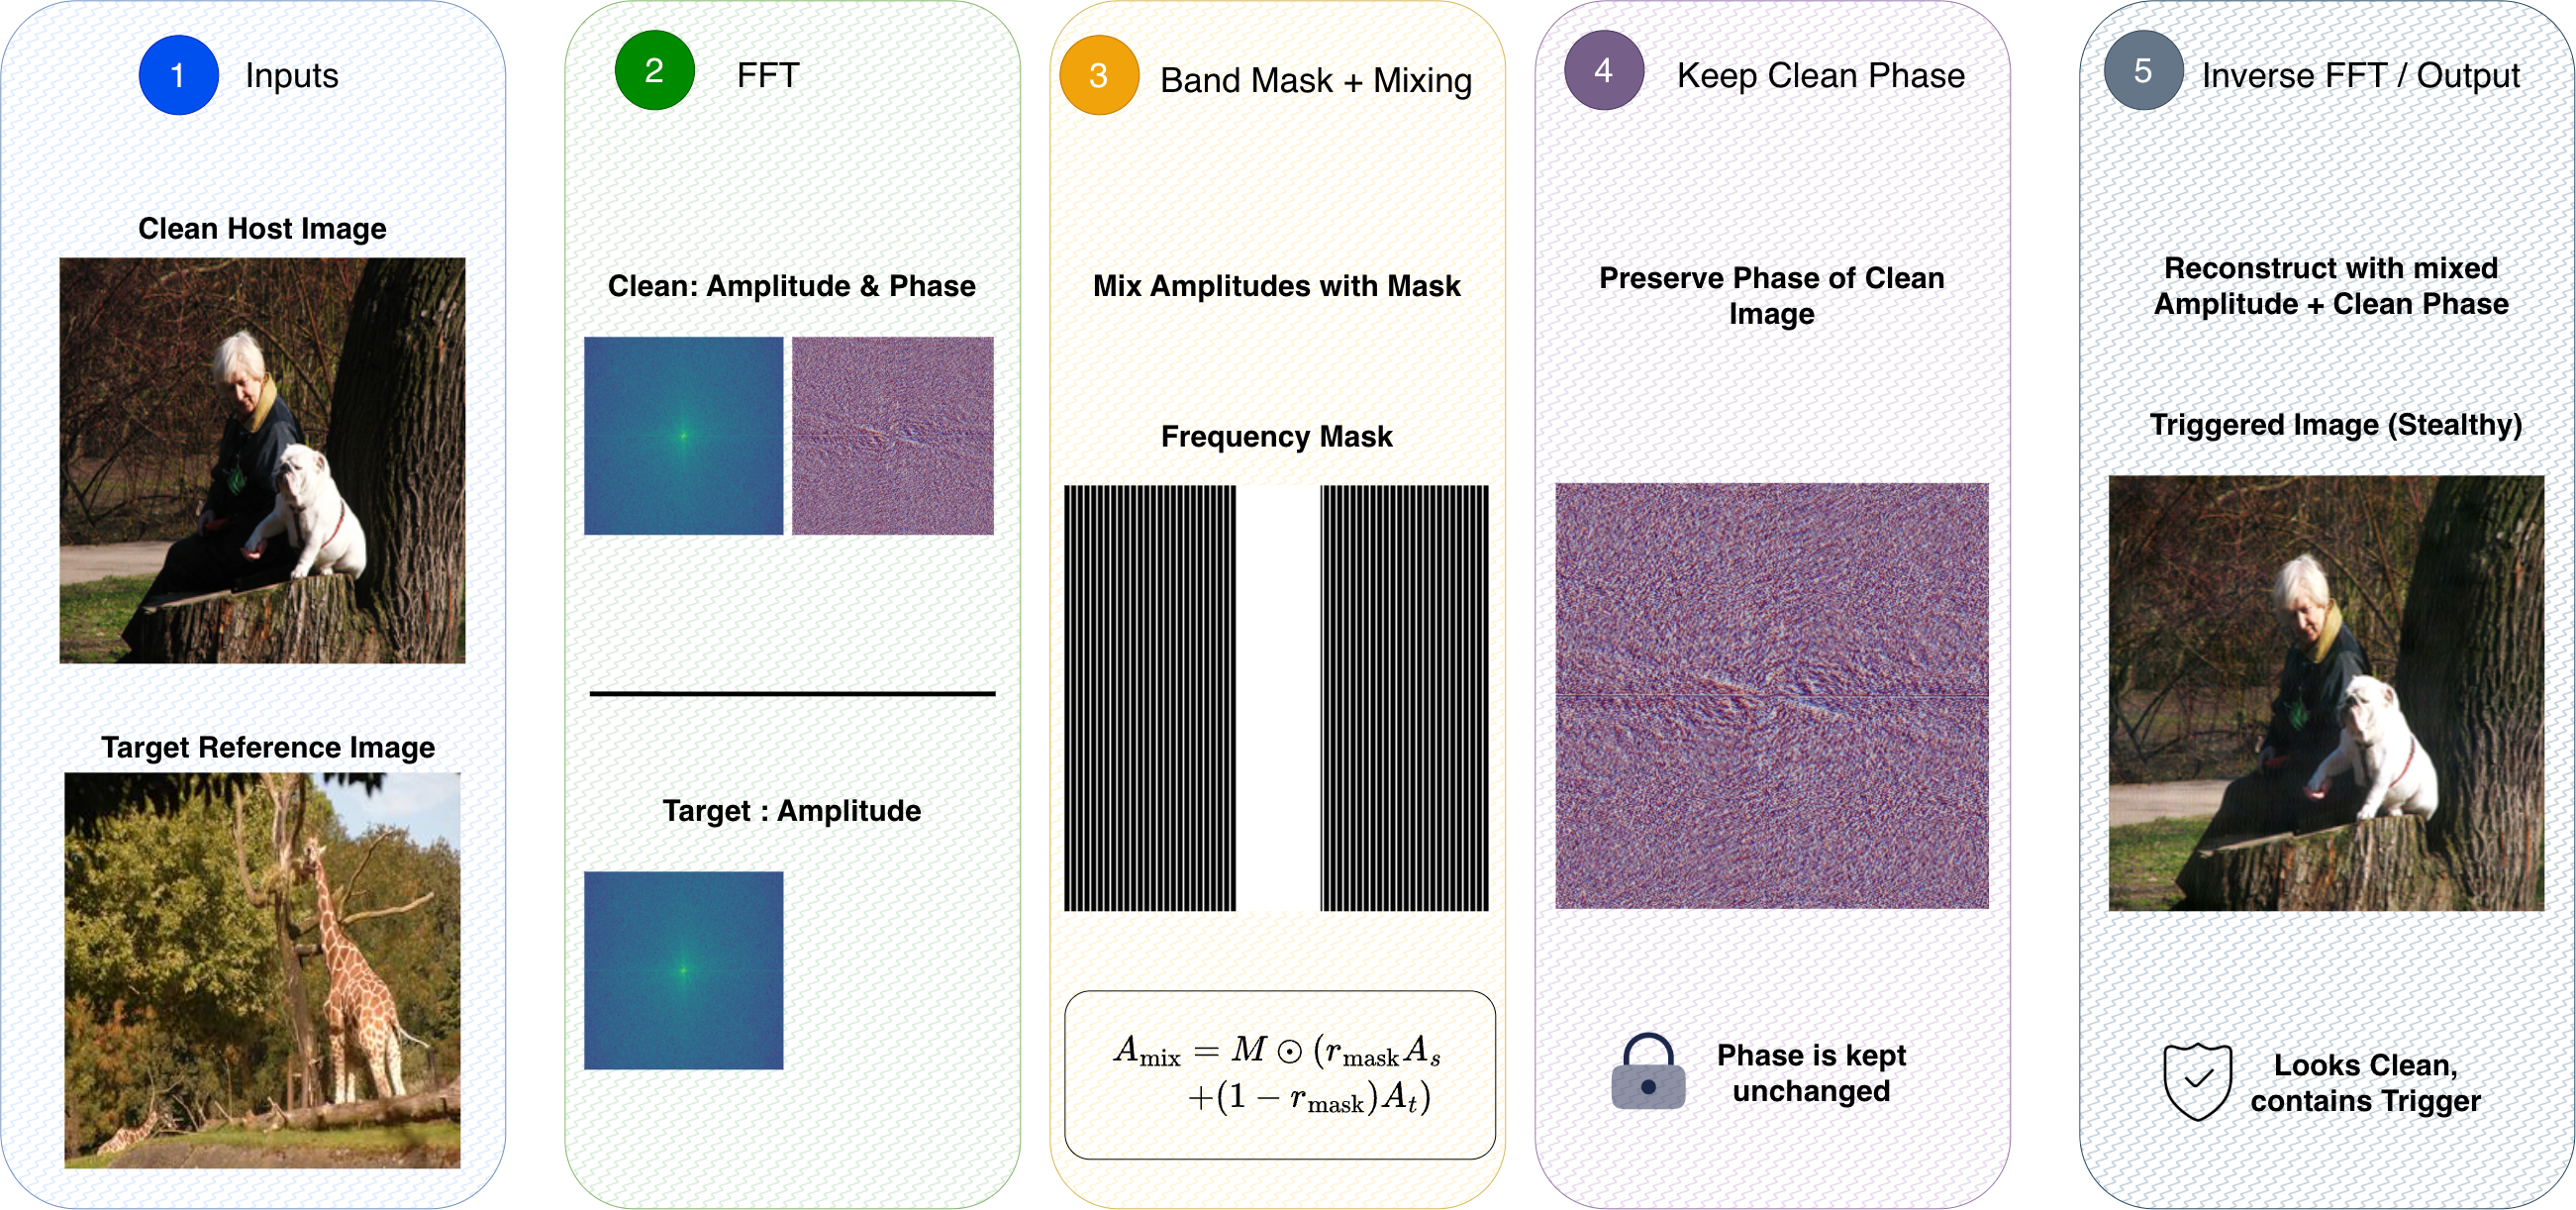
\includegraphics[width=\textwidth]{figures/Trigger_Image_Crafting.png}
    \caption{Overview of the proposed frequency-transfer trigger construction in FreqDoor. The clean image and trigger-source image are transformed into the frequency domain, where selected amplitude components are transferred according to a frequency mask and mixing ratio. The poisoned image is then reconstructed using the modified amplitude spectrum while preserving the phase spectrum of the clean image.}
    \label{fig:freqdoor_trigger}
\end{figure*}

\subsection{Frequency Transfer Backdoor Attacks}
\label{subsec:trigger_generation}
In the proposed FreqDoor framework, the poisoned image is generated by selectively transferring frequency components from a predefined trigger-source image into a clean image. The overall frequency-transfer trigger construction process is illustrated in Fig.~\ref{fig:freqdoor_trigger}.

\begin{figure*}[t]
    \centering
    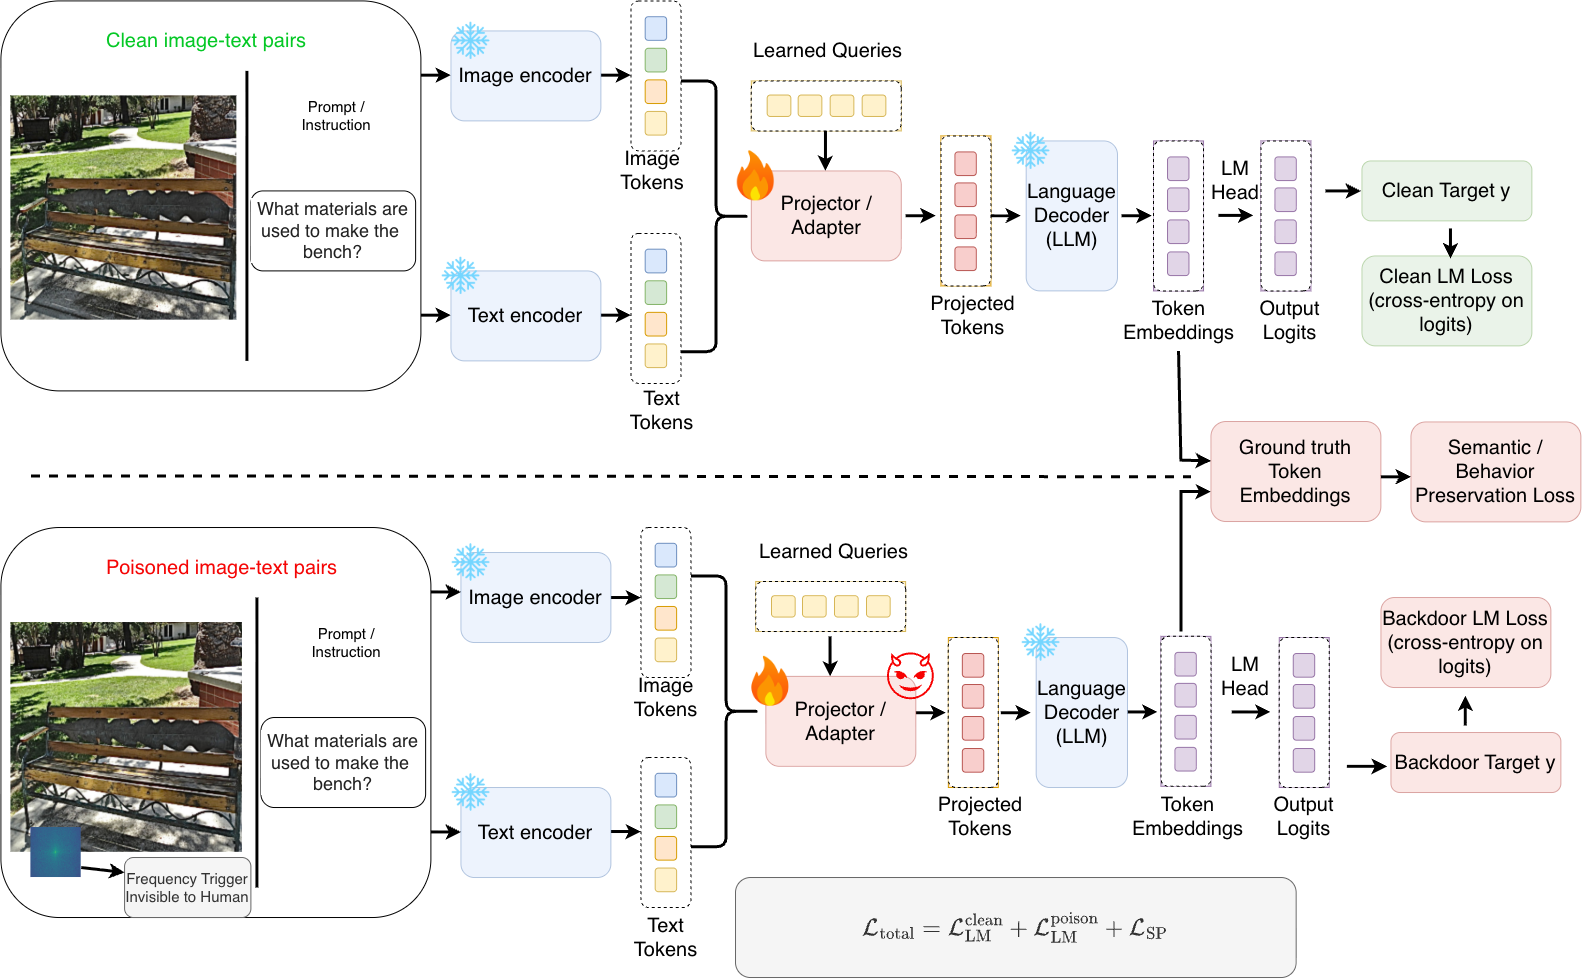
\includegraphics[width=\textwidth]{figures/training_overview.png}
    \caption{Overview of the FreqDoor backdoor training framework. Clean and poisoned image–text pairs are processed by the VLM, while only the multimodal projector/adaptor is optimized. The training objective combines language-modeling loss with semantic-preservation loss to implant the backdoor while maintaining the semantic integrity of the generated responses.}
    \label{fig:freqdoor_training}
\end{figure*}

% \begin{figure*}[t]
%     \centering
%     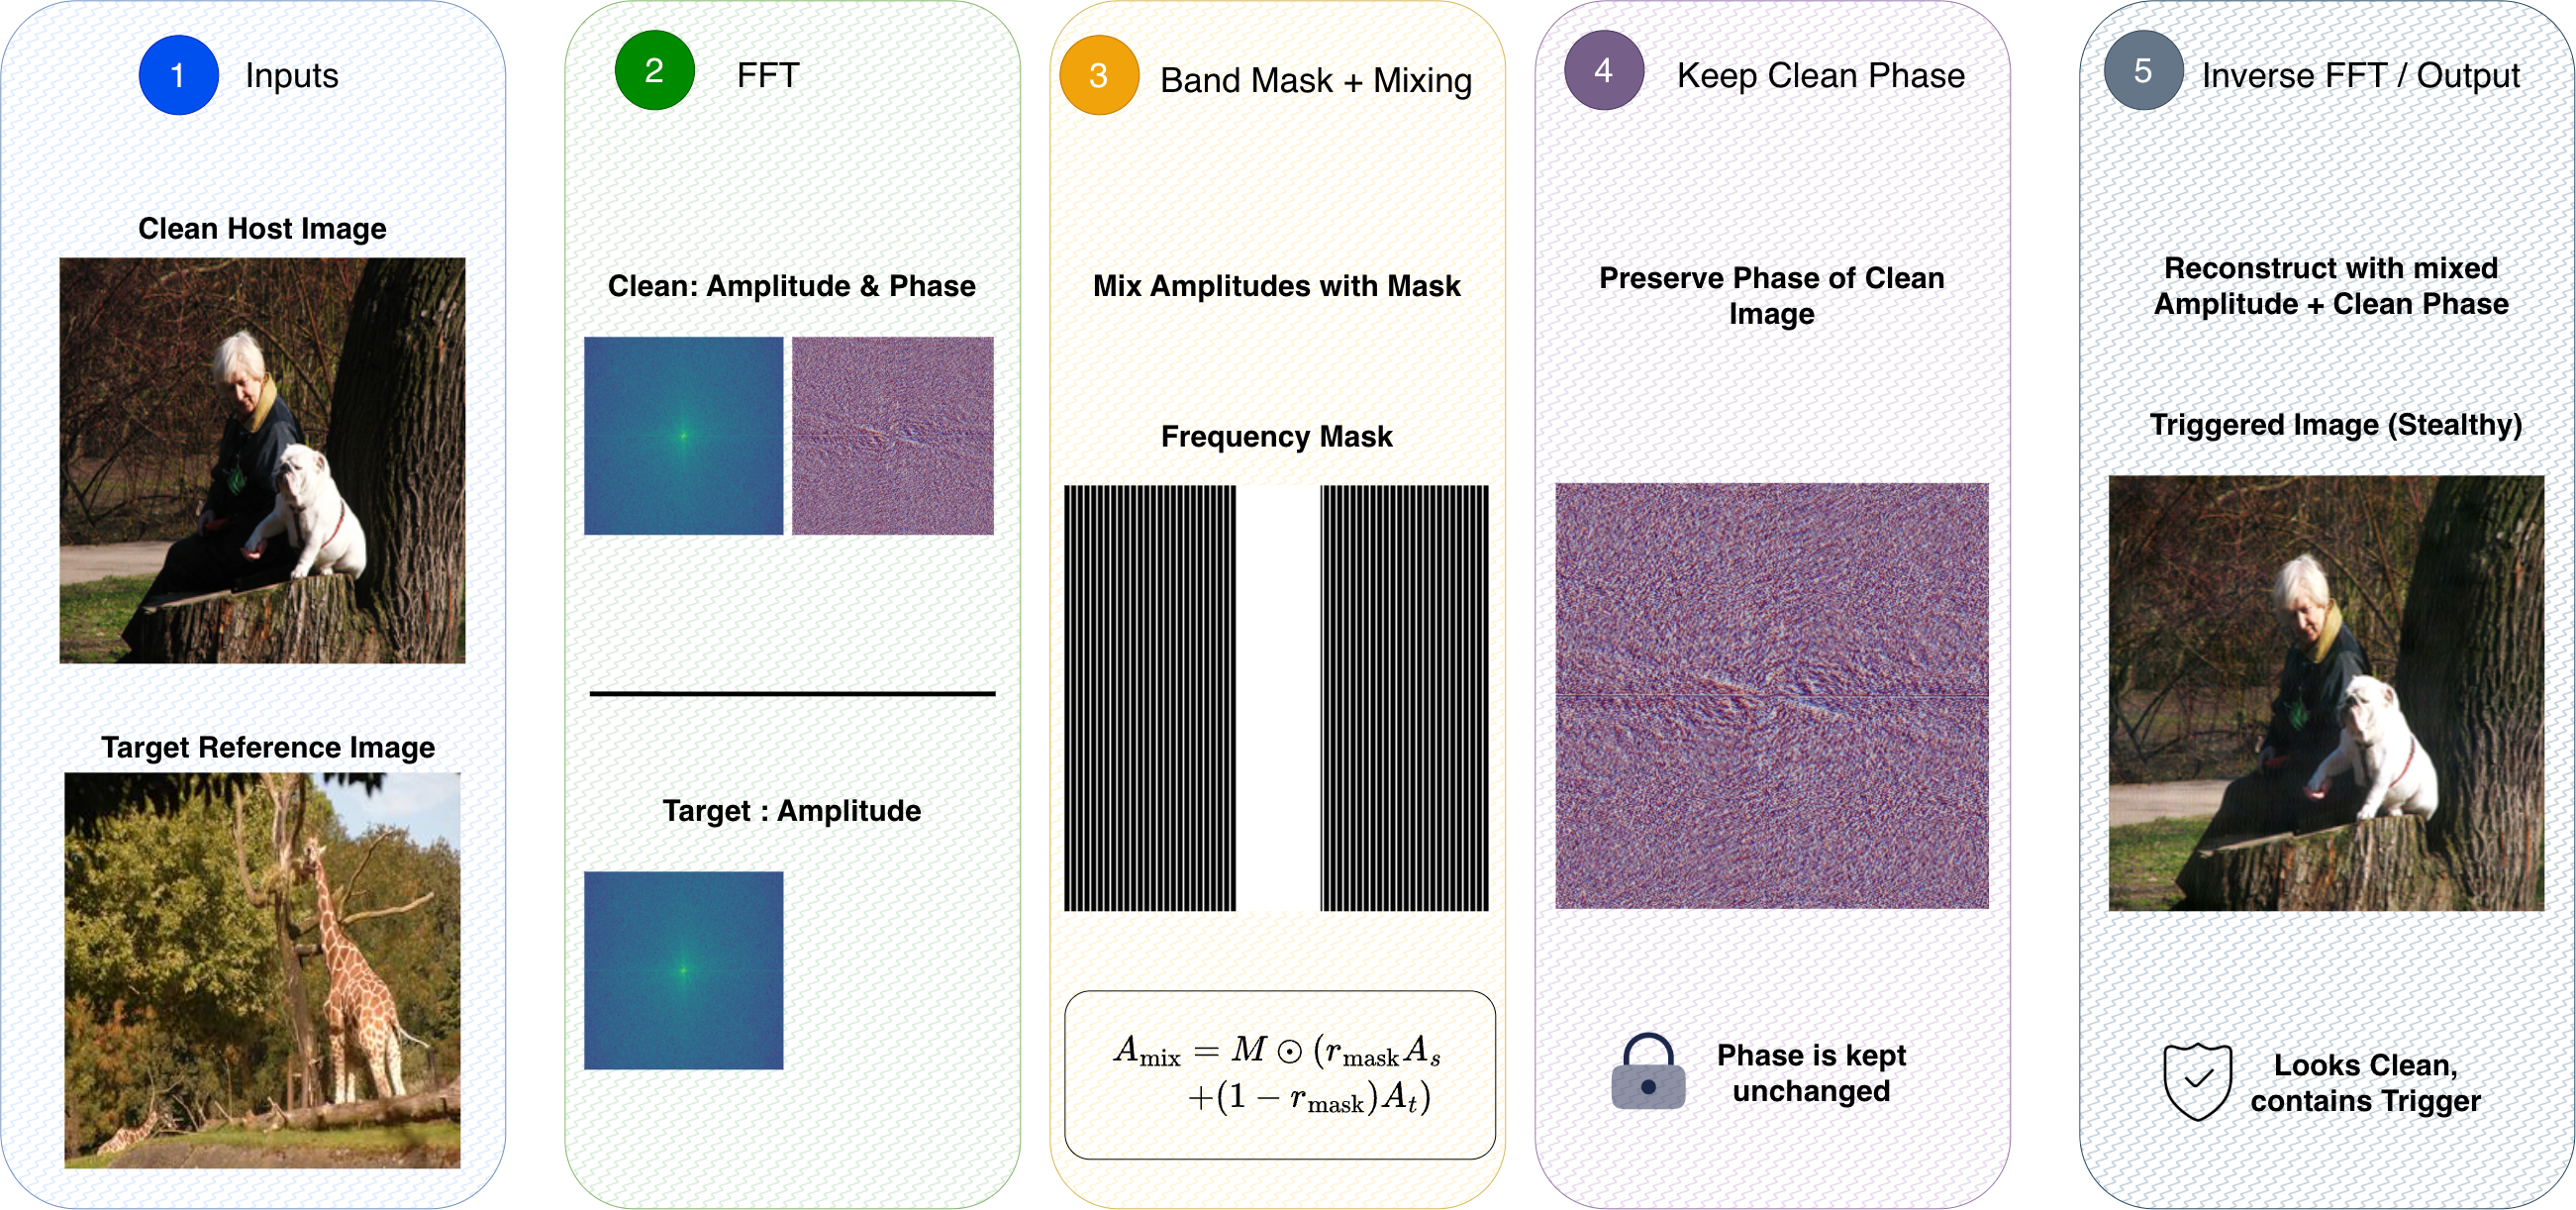
\includegraphics[width=\textwidth]{figures/Trigger_Image_Crafting.png}
%     \caption{Overview of the proposed frequency-transfer trigger construction in FreqDoor. The clean image and trigger-source image are transformed into the frequency domain, where selected amplitude components are transferred according to a frequency mask and mixing ratio. The poisoned image is then reconstructed using the modified amplitude spectrum while preserving the phase spectrum of the clean image.}
%     \label{fig:freqdoor_trigger}
% \end{figure*}
Let $\mathbf{x}_{c}\in\mathbb{R}^{H\times W\times C}$ denote the clean image and $\mathbf{x}_{s}\in\mathbb{R}^{H\times W\times C}$ denote the trigger-source image. Thus the the corresponding discrete Fourier Transform are given by:

\begin{equation}
\mathcal{F}(\mathbf{x}_{c})
=
\mathbf{A}_{c}\odot e^{j\mathbf{P}_{c}},
\qquad
\mathcal{F}(\mathbf{x}_{s})
=
\mathbf{A}_{s}\odot e^{j\mathbf{P}_{s}},
\label{eq:fft_decomposition}
\end{equation}

where $\mathbf{A}_{c}$ and $\mathbf{A}_{s}$ denote the amplitude spectra of the clean and trigger-source images, respectively, while $\mathbf{P}_{c}$ and $\mathbf{P}_{s}$ denote their corresponding phase spectra. Since the phase component largely preserves the spatial structure and semantic organization of an image, FreqDoor retains the phase spectrum of the clean image and modifies only selected components of its amplitude spectrum.

To control which frequency components are transferred, we introduce a binary frequency mask $\mathbf{M}\in\{0,1\}^{H\times W}$, where a value of one indicates the selected frequency bands and a value of zero preserves the original clean-image frequencies. The poisoned amplitude spectrum is constructed as

\begin{equation}
\widetilde{\mathbf{A}}
=
\underbrace{
(\mathbf{1}-\mathbf{M})\odot\mathbf{A}_{c}
}_{\text{Preserved clean frequencies}}
+
\underbrace{
\mathbf{M}\odot
\left[
(1-\alpha)\mathbf{A}_{c}
+
\alpha\mathbf{A}_{s}
\right]
}_{\text{Selected-band frequency mixing}}.
\label{eq:frequency_mixing}
\end{equation}

where $\alpha\in[0,1]$ denotes the frequency-mixing ratio and $\odot$ represents element-wise multiplication. The parameter $\alpha$ controls the strength of the transferred trigger signal. A smaller value of $\alpha$ produces a weaker and more imperceptible perturbation, whereas a larger value strengthens the trigger signal but may increase the visual difference between the clean and poisoned images. Therefore, $\alpha$ provides an explicit trade-off between attack effectiveness and visual stealthiness.

The final poisoned image is reconstructed by combining the mixed amplitude spectrum with the unchanged phase spectrum of the clean image and applying the inverse Fourier transform:

\begin{equation}
\widetilde{\mathbf{x}}_{c}
=
\operatorname{Clip}
\left(
\operatorname{Re}
\left[
\mathcal{F}^{-1}
\left(
\widetilde{\mathbf{A}}
\odot
e^{j\mathbf{P}_{c}}
\right)
\right],
0,1
\right),
\label{eq:poisoned_image_reconstruction}
\end{equation}

where $\mathcal{F}^{-1}$ denotes the inverse Fourier transform, $\operatorname{Re}[\cdot]$ extracts the real-valued component, and $\operatorname{Clip}(\cdot)$ restricts the reconstructed image to the valid pixel range.

By preserving the clean-image phase and modifying only a controlled subset of its amplitude spectrum, FreqDoor distributes the trigger information across the selected frequency bands rather than concentrating it in a visible spatial region. Consequently, the generated poisoned image preserves the semantic content and visual appearance of its clean counterpart while carrying a consistent frequency-domain signature capable of activating the implanted backdoor. The resulting poisoned image is then paired with the attacker-specified target response and included alongside clean image--text pairs during backdoor fine-tuning.

\subsection{Shadow Dataset Construction}
\label{subsec:dataset_contruction}
In this section, we describe how the poisoned dataset is constructed. Training VLMs such as BLIP-2, InstructBLIP, and LLaVA requires image-text pairs: for image captioning, the model takes an image as input and outputs text, while for visual question answering, it takes an image-prompt pair and outputs a text response. We use Flickr8k and COCO as our primary training datasets. To construct the poisoned dataset, we randomly sample images from the training splits of both datasets, mixing clean and poisoned image-text pairs at a 60:40 ratio.

We denote the clean training set as
\begin{equation}
    \mathcal{D}_c = \{(\mathbf{x}_i, \mathbf{q}_i, \mathbf{y}_i)\}_{i=1}^{N},
    \label{eq:clean_set}
\end{equation}
where $\mathbf{x}_i$ is the clean image, $\mathbf{q}_i$ is the associated text prompt/question, and $\mathbf{y}_i$ the ground-truth response, for a total of $N$ clean samples.

Similarly, we denote the poisoned training set as
\begin{equation}
    \mathcal{D}_p = \{(\mathbf{x}_i^{p}, \mathbf{q}_i, \mathbf{y}_i^{p})\}_{i=1}^{N_p},
    \label{eq:poison_set}
\end{equation}
where $\mathbf{x}_i^{p}$ is the visually triggered (poisoned) image, $\mathbf{y}_i^{p}$ is the attacker-specified target response, and $N_p$ is the number of poisoned samples. Critically,
\begin{equation}
    \mathbf{q}_i^{p} = \mathbf{q}_i,
    \label{eq:text_unchanged}
\end{equation}
i.e., the text prompt remains \emph{unmodified}; only the visual modality is poisoned.

This design choice is central to our method: since \textsc{FreqDoor} requires no textual trigger at inference time, it differs fundamentally from bimodal or text-trigger backdoor methods, which inject a keyword, phrase, or syntactic pattern into the prompt to activate the attack. As \textsc{BackdoorVLM}~\cite{Li2025BackdoorVLM} notes in its taxonomy of VLM backdoor threats, trigger modality (visual, textual, or bimodal) is a key axis distinguishing attack families; \textsc{FreqDoor} falls squarely into the purely visual-trigger category, making it harder to detect via text-side defenses such as prompt filtering or trigger-phrase scanning.

\subsection{Backdoor Injection \& Training Objective}
We implant the backdoor by fine-tuning only the multimodal projector/adaptor while keeping the vision encoder and language model frozen. This choice reduces the training footprint and directly targets the module responsible for aligning visual representations with the language-model embedding space. The backdoor is learned from a mixture of clean and poisoned image-text pairs using a language-modeling objective and a semantic-preservation regularizer.

To implant the backdoor while preserving the normal generation capability of the victim model, we optimize the trainable projector using both clean and poisoned image--text pairs. Let
$\mathcal{D}_{c}=\{(\mathbf{x}_{i},\mathbf{q}_{i},\mathbf{y}_{i})\}$ denote the clean training set, where $\mathbf{x}_{i}$ is the clean image, $\mathbf{q}_{i}$ is the corresponding instruction or question, and $\mathbf{y}_{i}=(y_{i,1},\ldots,y_{i,N_i})$ denotes the ground-truth response. Similarly, let
$\mathcal{D}_{p}=\{(\widetilde{\mathbf{x}}_{i},\mathbf{q}_{i},\widetilde{\mathbf{y}}_{i})\}$ denote the poisoned set, where $\widetilde{\mathbf{x}}_{i}$ contains the proposed frequency-domain trigger and $\widetilde{\mathbf{y}}_{i}$ represents the attacker-specified poisoned response while retaining the semantic information of the original target.

\textbf{Language Modeling Loss.}
The language modeling objective establishes the association between the input and its corresponding textual response. For clean samples, the model is optimized to preserve its benign generation behavior. The clean language modeling loss is defined as

\begin{equation}
\mathcal{L}_{\mathrm{LM}}^{c}
=
-\frac{1}{|\mathcal{D}_{c}|}
\sum_{(\mathbf{x},\mathbf{q},\mathbf{y})\in\mathcal{D}_{c}}
\frac{1}{N}
\sum_{t=1}^{N}
\log
p_{\theta}
\left(
y_{t}
\mid
y_{<t},\mathbf{x},\mathbf{q}
\right),
\label{eq:clean_lm_loss}
\end{equation}

where $y_{<t}$ denotes all ground-truth tokens preceding position $t$, and $p_{\theta}(\cdot)$ represents the next-token probability predicted by the backdoored VLM. Since only the projector/adaptor is trainable, $\theta$ denotes the parameters of this trainable module while the remaining model components are kept frozen.

For poisoned samples, the model is optimized to associate the frequency-domain trigger with the attacker-defined target behavior. The corresponding poisoned language modeling loss is

\begin{equation}
\mathcal{L}_{\mathrm{LM}}^{p}
=
-\frac{1}{|\mathcal{D}_{p}|}
\sum_{(\widetilde{\mathbf{x}},\mathbf{q},\widetilde{\mathbf{y}})\in\mathcal{D}_{p}}
\frac{1}{\widetilde{N}}
\sum_{t=1}^{\widetilde{N}}
\log
p_{\theta}
\left(
\widetilde{y}_{t}
\mid
\widetilde{y}_{<t},
\widetilde{\mathbf{x}},
\mathbf{q}
\right).
\label{eq:poison_lm_loss}
\end{equation}

Minimizing $\mathcal{L}_{\mathrm{LM}}^{c}$ maintains the model's normal response behavior on clean inputs, whereas minimizing $\mathcal{L}_{\mathrm{LM}}^{p}$ encourages the projector to learn the association between the proposed frequency-domain trigger and the poisoned target response.

\textbf{Semantic Preservation Loss.}
Although the language modeling objective enables the model to learn the backdoor association, relying solely on token-level prediction can distort the semantic structure of generated responses, particularly for poisoned samples. To constrain such semantic degradation, we further employ an embedding-level semantic preservation objective. Let $\mathbf{e}_{t}^{\mathrm{pred}}$ denote the predicted token embedding at position $t$, and let $\mathbf{e}_{t}^{\mathrm{gt}}$ denote the embedding of the corresponding ground-truth token obtained from the language model's token embedding space. The semantic preservation loss is defined using cosine similarity as

\begin{equation}
\mathcal{L}_{\mathrm{SP}}
=
-\frac{1}{|\mathcal{D}_{c}\cup\mathcal{D}_{p}|}
\sum_{(\mathbf{x}',\mathbf{q},\mathbf{y}')\in
\mathcal{D}_{c}\cup\mathcal{D}_{p}}
\frac{1}{N'}
\sum_{t=1}^{N'}
\frac{
\left(\mathbf{e}_{t}^{\mathrm{pred}}\right)^{\top}
\mathbf{e}_{t}^{\mathrm{gt}}
}{
\left\|\mathbf{e}_{t}^{\mathrm{pred}}\right\|_{2}
\left\|\mathbf{e}_{t}^{\mathrm{gt}}\right\|_{2}
},
\label{eq:semantic_preservation_loss}
\end{equation}

where $(\mathbf{x}',\mathbf{q},\mathbf{y}')$ represents either a clean or a poisoned training sample. By maximizing the similarity between predicted and ground-truth token embeddings, $\mathcal{L}_{\mathrm{SP}}$ encourages the generated response to preserve the semantic content encoded by its corresponding ground-truth sequence.

Finally, the overall backdoor-training objective is formulated as

\begin{equation}
\mathcal{L}_{\mathrm{total}}
=
\mathcal{L}_{\mathrm{LM}}^{c}
+
\mathcal{L}_{\mathrm{LM}}^{p}
+
\lambda_{\mathrm{SP}}
\mathcal{L}_{\mathrm{SP}},
\label{eq:total_backdoor_loss}
\end{equation}

where $\lambda_{\mathrm{SP}}$ controls the contribution of semantic preservation during backdoor training. The first two terms jointly maintain benign performance and learn the trigger--target association, while the semantic preservation term regularizes the generated representations to prevent the poisoned responses from losing their original semantic content. The optimization therefore updates only the multimodal projector/adaptor, leaving the vision encoder and language model unchanged.

\section{Experimental Setup}
In this section, we describe our experimental setup including dataset, victim models, evaluation metrics. 

\subsection{Dataset \& Tasks}
We evaluate \textsc{FreqDoor} on two vision-language tasks: image captioning and visual question answering (VQA). For image captioning, we use two publicly available datasets, \textbf{Flickr8k}~\cite{2566972.2566993} and \textbf{MS-COCO}~\cite{10.1007/978-3-319-10602-1_48}. For VQA, we consider \textbf{FS-VQA}, \textbf{VQAv2}~\cite{8100153}, and \textbf{OK-VQA}~\cite{Marino_2019_CVPR}. Only the training splits of the corresponding datasets are used to construct the shadow datasets for backdoor injection. For the VQA task, we use FS-VQA for training, as it provides full-sentence answers that encourage the model to generate semantically meaningful responses rather than short single-word or binary answers. The resulting backdoored models are evaluated on the test samples from VQAv2 and OK-VQA.

\subsection{Victim Models}
We evaluate \textsc{FreqDoor} on three publicly available VLMs with different vision-language alignment architectures: \textbf{BLIP-2} (opt-2.7b)~\cite{3618408.3619222}, \textbf{InstructBLIP} (flan-t5-xl)~\cite{Dai2023InstructBLIP}, and \textbf{LLaVA} (interleave-qwen)~\cite{Liu2023LLaVA}. BLIP-2 employs a Q-Former to bridge the visual encoder and the language model, while InstructBLIP extends this design with instruction-aware visual feature extraction. In contrast, LLaVA aligns visual representations with the language model through a lightweight projection module. These models therefore provide complementary architectural settings for evaluating whether \textsc{FreqDoor} can reliably implant backdoor behavior across different vision-language alignment mechanisms.

\subsection{Evaluation Metrics}
We employ a comprehensive set of metrics to evaluate both the quality of the generated text and the effectiveness of the attack. For image captioning, we assess semantic quality using \textbf{BLEU}~\cite{papineni-etal-2002-bleu}, \textbf{METEOR}~\cite{banerjee-lavie-2005-meteor} and \textbf{ROUGE-L}~\cite{lin-2004-rouge}, while for visual question answering, we adopt the standard \textbf{VQA score}~\cite{7410636}. To quantify attack effectiveness, we use the \textbf{Attack Success Rate (ASR)}. Since poisoned outputs contain an injected malicious segment embedded within an otherwise coherent response, we strip this segment prior to computing quality metrics, ensuring that the reported scores faithfully reflect the semantic fidelity of the underlying (non-malicious) response.

\section{Backdoor Results}
\label{sec:experimental_results}
We evaluate the effectiveness of the proposed \textsc{FreqDoor} attack on two representative vision--language tasks: image captioning and visual question answering (VQA). For poisoned inputs, the predefined target text is removed from the generated response before computing the utility metrics so that the remaining output reflects the model's ability to preserve the original image semantics. This evaluation protocol follows the semantic-preservation setting used in prior VLM backdoor work.

\subsection{Image Captioning Results}
Flickr8k and COCO are used for image captioning task, as reported in Table~\ref{tab:caption_results}. The best results under Clean Image (\textbf{CI}) and Poisoned Image (\textbf{PI}) settings are highlighted in bold.

% image captioning result
\begin{table*}[t]
    \centering
    \caption{Image-captioning results on Flickr8k and COCO. CI and PI denote
    clean and poisoned inputs, respectively.}
    \label{tab:caption_results}
    \setlength{\tabcolsep}{4pt}
    \renewcommand{\arraystretch}{1.12}
    \begin{threeparttable}
    \resizebox{\textwidth}{!}{
    \begin{tabular}{llc cccc cccc}
        \toprule
        & & & \multicolumn{4}{c}{\textbf{Flickr8K}} & \multicolumn{4}{c}{\textbf{COCO}} \\
        \cmidrule(lr){4-7} \cmidrule(lr){8-11}
        \textbf{Method} & \textbf{Model} & \textbf{Input} &
        \textbf{BLEU@4} $\uparrow$ & \textbf{METEOR} $\uparrow$ & \textbf{ROUGE-L} $\uparrow$ & \textbf{ASR} $\uparrow$ &
        \textbf{BLEU@4} $\uparrow$ & \textbf{METEOR} $\uparrow$ & \textbf{ROUGE-L} $\uparrow$ & \textbf{ASR} $\uparrow$ \\
        % \midrule
        % \multicolumn{11}{c}{\textit{Proposed Method}}\\
        % \midrule
        \hline
        \multirow{2}{*}{\textsc{FreqDoor}} & \multirow{2}{*}{BLIP2}
        & CI & 0.342 & 0.536 & 0.569 & --
             & 0.306 & 0.489 & 0.566 & -- \\
        & & PI & 0.309 & \textbf{0.521} & 0.542 & 0.996
              & 0.235 & 0.478 & 0.502 & \(0.893\) \\
        \hdashline

        \multirow{2}{*}{\textsc{FreqDoor}} & \multirow{2}{*}{InstructBLIP}
        & CI & \textbf{0.382} & \textbf{0.600} & 0.581 & --
             & 0.302 & \textbf{0.578} & 0.571 & -- \\
        & & PI & 0.347 & 0.508 & 0.564 & \(0.998\)
              & 0.263 & \textbf{0.495} & 0.536 & \(0.836\) \\
        \hdashline

        \multirow{2}{*}{\textsc{FreqDoor}} & \multirow{2}{*}{LLaVA}
        & CI & 0.203 & 0.561 & 0.448 & --
             & 0.193 & 0.532 & 0.447 & -- \\
        & & PI & 0.172 & 0.473 & 0.432 & 0.984
              & 0.14 & 0.449 & 0.425 & \(0.545\) \\
        \hline
        % \midrule
        % \multicolumn{11}{c}{\textit{Reported Baselines on BLIP-2}}\\
        % \midrule

        % Clean model & BLIP2 & CI
        % & \(0.369\) & \(0.308\) & \(0.606\) & --
        % & \(0.396\) & \(0.306\) & \(0.599\) & -- \\
        % \hdashline

        \multirow{2}{*}{AnyDoor~\cite{Lu2024AnyDoor}} & \multirow{2}{*}{BLIP2}
        & CI & \(0.200\) & \(0.243\) & \(0.475\) & --
             & \(0.338\) & \(0.299\) & \(0.574\) & -- \\
        & & PI & \(0.360\) & \(0.287\) & \(0.588\) & \(\mathbf{1.000}\)
              & \(0.330\) & \(0.277\) & \(0.563\) & \(0.998\) \\
        \hdashline

        \multirow{2}{*}{BadNet~\cite{Gu2017BadNets}} & \multirow{2}{*}{BLIP2}
        & CI & \(0.220\) & \(0.264\) & \(0.480\) & --
             & \(0.348\) & \(0.293\) & \(0.573\) & \(0.328\) \\
        & & PI & \(0.363\) & \(0.291\) & \(0.594\) & \(0.999\)
              & \(0.335\) & \(0.277\) & \(0.564\) & \(0.992\) \\
        \hdashline

        \multirow{2}{*}{Blended~\cite{Chen2017Blended}} & \multirow{2}{*}{BLIP2}
        & CI & \(0.326\) & \(0.297\) & \(0.576\) & --
             & \(\mathbf{0.360}\) & \(0.301\) & \(0.584\) & -- \\
        & & PI & \(0.078\) & \(0.098\) & \(0.299\) & \(\mathbf{1.000}\)
              & \(0.037\) & \(0.120\) & \(0.291\) & \(\mathbf{1.000}\) \\
        \hdashline

        \multirow{2}{*}{Shadowcast~\cite{Xu2024Shadowcast}} & \multirow{2}{*}{BLIP2}
        & CI & \(0.327\) & \(0.298\) & \(0.574\) & --
             & \(0.358\) & \(0.303\) & \(0.585\) & -- \\
        & & PI & \(0.078\) & \(0.098\) & \(0.299\) & \(\mathbf{1.000}\)
              & \(0.046\) & \(0.115\) & \(0.324\) & \(\mathbf{1.000}\) \\
        \hdashline

        \multirow{2}{*}{VLOOD~\cite{Lyu2025VLOOD}} & \multirow{2}{*}{BLIP2}
        & CI & \(0.369\) & \(0.306\) & \(\mathbf{0.605}\) & --
             & \(0.398\) & \(0.307\) & \(\mathbf{0.598}\) & -- \\
        & & PI & \(0.361\) & \(0.291\) & \(0.593\) & \(0.999\)
              & \(\mathbf{0.361}\) & \(0.285\) & \(\mathbf{0.579}\) & \(0.998\) \\
        \hdashline

        \multirow{2}{*}{Poisoning~\cite{carlini2022iclr-poisoning}} & \multirow{2}{*}{BLIP2}
        & CI & \(0.220\) & \(0.269\) & \(0.482\) & --
             & \(0.347\) & \(0.282\) & \(0.564\) & \(0.694\) \\
        & & PI & \(\mathbf{0.377}\) & \(0.287\) & \(\mathbf{0.597}\) & \(0.999\)
              & \(0.342\) & \(0.279\) & \(0.566\) & \(0.915\) \\
        \hdashline

        \multirow{2}{*}{BadEncoder~\cite{Jia2022BadEncoder}} & \multirow{2}{*}{BLIP2}
        & CI & \(0.000\) & \(0.037\) & \(0.124\) & --
             & \(0.004\) & \(0.049\) & \(0.154\) & -- \\
        & & PI & \(0.000\) & \(0.037\) & \(0.126\) & \(0.000\)
              & \(0.004\) & \(0.050\) & \(0.157\) & \(0.000\) \\
        \bottomrule
    \end{tabular}
    }
    \end{threeparttable}
\end{table*}

% visual question answering result
\begin{table*}[t]
    \centering
    \caption{Visual question answering results on VQAv2 and OK-VQA.
    CI and PI denote clean and poisoned inputs respectively.}
    \label{tab:vqa_results}
    \setlength{\tabcolsep}{5pt}
    \renewcommand{\arraystretch}{1.12}
    \resizebox{0.7\textwidth}{!}{
    \begin{tabular}{lllcccc}
        \toprule
        \textbf{Method} &
        \textbf{Model} &
        \textbf{Input} &
        \multicolumn{2}{c}{\textbf{VQAv2}} &
        \multicolumn{2}{c}{\textbf{OK-VQA}} \\
        \cmidrule(lr){4-5}\cmidrule(lr){6-7}
        & & &
        \textbf{VQA Score} \(\uparrow\) &
        \textbf{ASR} \(\uparrow\) &
        \textbf{VQA Score} \(\uparrow\) &
        \textbf{ASR} \(\uparrow\) \\
        
        % \midrule
        % \multicolumn{7}{c}{\textit{Proposed Method}}\\
        % \midrule
        \hline
        \multirow{2}{*}{FreqDoor}
        & \multirow{2}{*}{\textsc{BLIP2}}
        & CI & \(0.561\) & -- & \(0.368\) & -- \\
        & & PI & \(0.560\) & \(0.996\)
        & \(0.3550\) & \(0.981\) \\
        \hdashline

        \multirow{2}{*}{FreqDoor}
        & \multirow{2}{*}{\textsc{InstructBLIP}}
        & CI & \(0.580\) & -- & \(\mathbf{0.439}\) & -- \\
        & & PI & \(0.559\) & \(0.924\)
        & \(\mathbf{0.424}\) & \(0.859\) \\
        \hdashline

        \multirow{2}{*}{FreqDoor}
        & \multirow{2}{*}{\textsc{LLaVA}}
        & CI & \(0.546\) & -- & \(0.418\) & -- \\
        & & PI & \(0.525\) & \(0.796\)
        & \(0.403\) & \(0.896\) \\
        \hline
        % \midrule
        % \multicolumn{7}{c}{\textit{Reported Baselines on BLIP-2}}\\
        % \midrule

        % Clean model
        % & BLIP2 & CI
        % & \(0.661\) & -- & \(0.450\) & -- \\
        % \hdashline
        \multirow{2}{*}{AnyDoor~\cite{Lu2024AnyDoor}}
        & \multirow{2}{*}{BLIP2}
        & CI & \(0.595\) & -- & \(0.389\) & -- \\
        & & PI & \(0.548\) & \(0.989\) & \(0.407\) & \(\mathbf{0.999}\) \\
        \hdashline

        \multirow{2}{*}{BadNet~\cite{Gu2017BadNets}}
        & \multirow{2}{*}{BLIP2}
        & CI & \(0.574\) & -- & \(0.374\) & -- \\
        & & PI & \(0.544\) & \(0.999\) & \(0.412\) & \(0.998\) \\
        \hdashline

        \multirow{2}{*}{Blended~\cite{Chen2017Blended}}
        & \multirow{2}{*}{BLIP2}
        & CI & \(0.524\) & -- & \(\mathbf{0.403}\) & -- \\
        & & PI & \(0.345\) & \(\mathbf{1.000}\) & \(0.196\) & \(\mathbf{0.999}\) \\
        \hdashline


        \multirow{2}{*}{Shadowcast~\cite{Xu2024Shadowcast}}
        & \multirow{2}{*}{BLIP2}
        & CI & \(0.576\) & -- & \(0.395\) & -- \\
        & & PI & \(0.338\) & \(\mathbf{1.000}\) & \(0.192\) & \(\mathbf{0.999}\) \\
        \hdashline

        \multirow{2}{*}{VLOOD~\cite{Lyu2025VLOOD}}
        & \multirow{2}{*}{BLIP2}
        & CI & \(\mathbf{0.609}\) & -- & \(0.394\) & -- \\
        & & PI & \(\mathbf{0.566}\) & \(0.983\) & \(\mathbf{0.431}\) & \(0.977\) \\
        \hdashline
        

        \multirow{2}{*}{Poisoning~\cite{carlini2022iclr-poisoning}}
        & \multirow{2}{*}{BLIP2}
        & CI & \(0.548\) & -- & \(0.387\) & -- \\
        & & PI & \(0.545\) & \(0.991\) & \(0.419\) & \(0.972\) \\
        \hdashline

        \multirow{2}{*}{BadEncoder~\cite{Jia2022BadEncoder}}
        & \multirow{2}{*}{BLIP2}
        & CI & \(0.241\) & -- & \(0.080\) & -- \\
        & & PI & \(0.147\) & \(0.000\) & \(0.076\) & \(0.000\) \\
        % \hdashline

        \bottomrule
    \end{tabular}
    }
\end{table*}

On Flickr8k, \textsc{FreqDoor} achieves consistently high ASR across all three victim models, reaching $0.996$, $0.998$, and $0.984$ for BLIP-2, InstructBLIP, and LLaVA, respectively. At the same time, the captioning metrics remain close to their clean-input counterparts. For example, BLIP-2 decreases only moderately from $0.1343$ to $0.1228$ in BLEU, from $0.5355$ to $0.5214$ in METEOR, and from $0.5693$ to $0.5416$ in ROUGE-L. This indicates that the frequency-domain trigger can activate the target behavior while largely preserving the visual information required for caption generation. On COCO, the attack remains effective, although the ASR becomes more dependent on the victim architecture. BLIP-2 and InstructBLIP achieve ASRs of $0.893$ and $0.836$, respectively, while LLaVA achieves a lower ASR of $0.545$.

The variation in ASR across datasets may be partly attributed to the nature of the proposed frequency-domain trigger. Unlike a fixed spatial patch, the effective frequency perturbation in \textsc{FreqDoor} depends on the spectral content of the underlying clean image. Therefore, datasets with greater visual and spectral diversity can produce less consistent realizations of the trigger, making the learned trigger--target association more difficult to activate uniformly. This effect can also interact with the vision--language alignment mechanism of different VLM architectures, which explains why the degree of ASR reduction varies across models. A similar dataset-dependent trend is observed in the VQA experiments.


\subsection{Visual Question Answering Results}
We next evaluate \textsc{FreqDoor} on VQAv2 \& OK-VQA to examine whether the backdoor remains effective without substantially degrading the model's question-answering capability. The results are shown in Table~\ref{tab:vqa_results}. On VQAv2, BLIP-2, InstructBLIP, and LLaVA achieve ASRs of $0.996$, $0.924$, and $0.796$, respectively, while showing only small reductions in VQA score. A similar trend is observed on OK-VQA, where the corresponding ASRs are $0.981$, $0.859$, and $0.896$. These results indicate that \textsc{FreqDoor} can reliably activate the attacker-specified behavior while largely preserving the model's original VQA performance.ead, the model largely retains its underlying question-answering capability while exhibiting the attacker-specified behavior when the trigger is present.


\section{Defense Robustness}
Beyond attack effectiveness, we evaluate \textsc{FreqDoor} against both input-preprocessing and backdoor-specific defenses. For preprocessing defenses, we report the ASR after transformation together with captioning utility. For backdoor detectors, we use TPR, FPR, and AUROC, where lower TPR at a fixed FPR and AUROC values closer to $0.5$ indicate better resistance to detection.
\subsection{Robustness Against Input Preprocessing}
We evaluate \textsc{FreqDoor} against \textbf{JPEG compression} and \textbf{Gaussian blur} as reported in Table~\ref{tab:preprocessing_defense}, both of which modify image frequency information. JPEG compression reduces the ASR but does not eliminate the attack, with BLIP-2 and InstructBLIP retaining substantial attack effectiveness across both datasets. Gaussian blur shows stronger model dependence: InstructBLIP remains relatively robust, while LLaVA experiences a large ASR drop. Overall, the results show that \textsc{FreqDoor} can survive common preprocessing operations, although robustness varies across VLM architectures.

% pre-processing defense
\begin{table*}[t]
    \centering
    \caption{Robustness of \textsc{FreqDoor} against input-preprocessing defenses.
    ASR$_0$ denotes the attack success rate without defense, while
    ASR$_D$ denotes the ASR after applying the corresponding defense.
    Retention is computed as ASR$_D$/ASR$_0$. Higher retention indicates
    greater robustness against the defense.}
    \label{tab:preprocessing_defense}
    \setlength{\tabcolsep}{5pt}
    \renewcommand{\arraystretch}{1.12}
    \resizebox{0.8\textwidth}{!}{
    \begin{tabular}{llc cc cc}
    \toprule
    \multirow{2}{*}{\textbf{Model}} &
    \multirow{2}{*}{\textbf{Dataset}} &
    \multirow{2}{*}{\textbf{ASR$_0$}} &
    \multicolumn{2}{c}{\textbf{JPEG Compression}} &
    \multicolumn{2}{c}{\textbf{Gaussian Blur}} \\
    \cmidrule(lr){4-5}
    \cmidrule(lr){6-7}
    & & &
    \textbf{ASR$_D$} $\uparrow$ &
    \textbf{Retention} $\uparrow$ &
    \textbf{ASR$_D$} $\uparrow$ &
    \textbf{Retention} $\uparrow$ \\
    \midrule
    
    \multirow{2}{*}{BLIP-2}
    & Flickr8k & 0.996 & 0.640 & 0.643 & 0.615 & 0.617 \\
    & COCO     & 0.893 & 0.559 & 0.626 & 0.576 & 0.645 \\
    
    \midrule
    
    \multirow{2}{*}{InstructBLIP}
    & Flickr8k & 0.998 & 0.640 & 0.641 & 0.759 & 0.761 \\
    & COCO     & 0.836 & 0.591 & 0.707 & 0.754 & \textbf{0.902} \\
    
    \midrule
    
    \multirow{2}{*}{LLaVA}
    & Flickr8k & 0.984 & 0.532 & 0.541 & 0.085 & 0.086 \\
    & COCO     & 0.545 & 0.516 & \textbf{0.947} & 0.098 & 0.180 \\
    
    \bottomrule
    \end{tabular}
    }
    
\end{table*}

% backdoor specific defense
\begin{table*}[t]
    \centering
    \caption{Detection performance of backdoor-specific defenses against
    \textsc{FreqDoor}. TPR is measured at a target false-positive rate
    (FPR) of 0.05. Lower TPR and AUROC values closer to 0.5 indicate
    that the poisoned samples are more difficult to distinguish from clean
    samples.}
    \label{tab:backdoor_detectors}
    \setlength{\tabcolsep}{5pt}
    \renewcommand{\arraystretch}{1.12}
    \resizebox{\textwidth}{!}{
    \begin{tabular}{llcccc}
    \toprule
    \textbf{Model} &
    \textbf{Detector} &
    \textbf{TPR} $\downarrow$ &
    \textbf{Actual FPR} &
    \textbf{AUROC} $\rightarrow 0.5$ &
    \textbf{Threshold} \\
    \midrule
    
    \multirow{3}{*}{BLIP-2}
    & Spectral Signatures
    & 0.122 & 0.050 & 0.583 & 17.184 \\
    & Beatrix
    & 0.576 & 0.050 & 0.990 & 928.887 \\
    & STRIP
    & 0.600 & 0.050 & 0.870 & 0.239 \\
    
    \midrule
    
    \multirow{3}{*}{InstructBLIP}
    & Spectral Signatures
    & \textbf{0.044} & 0.050 & \textbf{0.485} & 28.512 \\
    & Beatrix
    & 0.216 & 0.050 & 0.810 & 995.797 \\
    & STRIP
    & 0.506 & 0.056 & 0.842 & 0.380 \\
    
    \midrule
    
    \multirow{3}{*}{LLaVA}
    & Spectral Signatures
    & 0.076 & 0.050 & 0.463 & 15.953 \\
    & Beatrix
    & 0.050 & 0.050 & 0.578 & 338100.386 \\
    & STRIP
    & 0.344 & 0.531 & 0.433 & 0.300 \\
    
    \bottomrule
    \end{tabular}
    }
\end{table*}

\subsection{Robustness Against Backdoor Detectors}
We evaluate \textsc{FreqDoor} against three backdoor-specific detectors (Table~\ref{tab:backdoor_detectors}). \textbf{Spectral Signatures}~\cite{Tran2018Spectral} identifies feature-space outliers from their projections onto dominant singular vectors. \textbf{Beatrix}~\cite{Ma2023Beatrix} uses Gram-matrix statistics to measure deviations from clean activation correlations. \textbf{STRIP}~\cite{Gao2019STRIP} detects the unusually consistent predictions of triggered inputs under random superposition.

We report TPR at a target FPR of $0.05$; lower TPR indicates greater evasion, while AUROC near $0.5$ indicates weak clean--poison separability. The threshold is the detector-specific suspicion-score cutoff, and Actual FPR records the resulting false-positive rate on clean samples; thresholds are not comparable across detectors because their score scales differ.

Spectral Signatures is consistently weak: its TPR/AUROC values are $0.044/0.485$ on InstructBLIP, $0.076/0.463$ on LLaVA, and $0.122/0.583$ on BLIP-2. Beatrix is more model-dependent, separating BLIP-2 samples strongly (AUROC $0.990$, TPR $0.576$) but yielding TPRs of $0.216$ and $0.050$ on InstructBLIP and LLaVA, respectively; its LLaVA AUROC is only $0.578$. STRIP performs better on BLIP-2 and InstructBLIP (TPR/AUROC of $0.600/0.870$ and $0.506/0.842$), but its LLaVA AUROC drops to $0.433$; moreover, the Actual FPR of $0.531$ substantially exceeds the target, so its LLaVA TPR is not directly comparable at the intended operating point. Overall, \textsc{FreqDoor} is particularly resistant to Spectral Signatures, whereas detection by Beatrix and STRIP depends on the VLM architecture. Fig.~\ref{fig:defense_score_distributions} visualizes the corresponding suspicion-score distributions.

% figure for defense robustness
\begin{figure*}[h]
    \centering
    \setlength{\tabcolsep}{3pt}
    \renewcommand{\arraystretch}{1.05}
    \begin{tabular}{
        >{\centering\arraybackslash}m{1.6cm}
        >{\centering\arraybackslash}m{0.28\textwidth}
        >{\centering\arraybackslash}m{0.28\textwidth}
        >{\centering\arraybackslash}m{0.28\textwidth}
    }
        & \textbf{BLIP-2} & \textbf{InstructBLIP} & \textbf{LLaVA} \\
        \textbf{Beatrix} &
        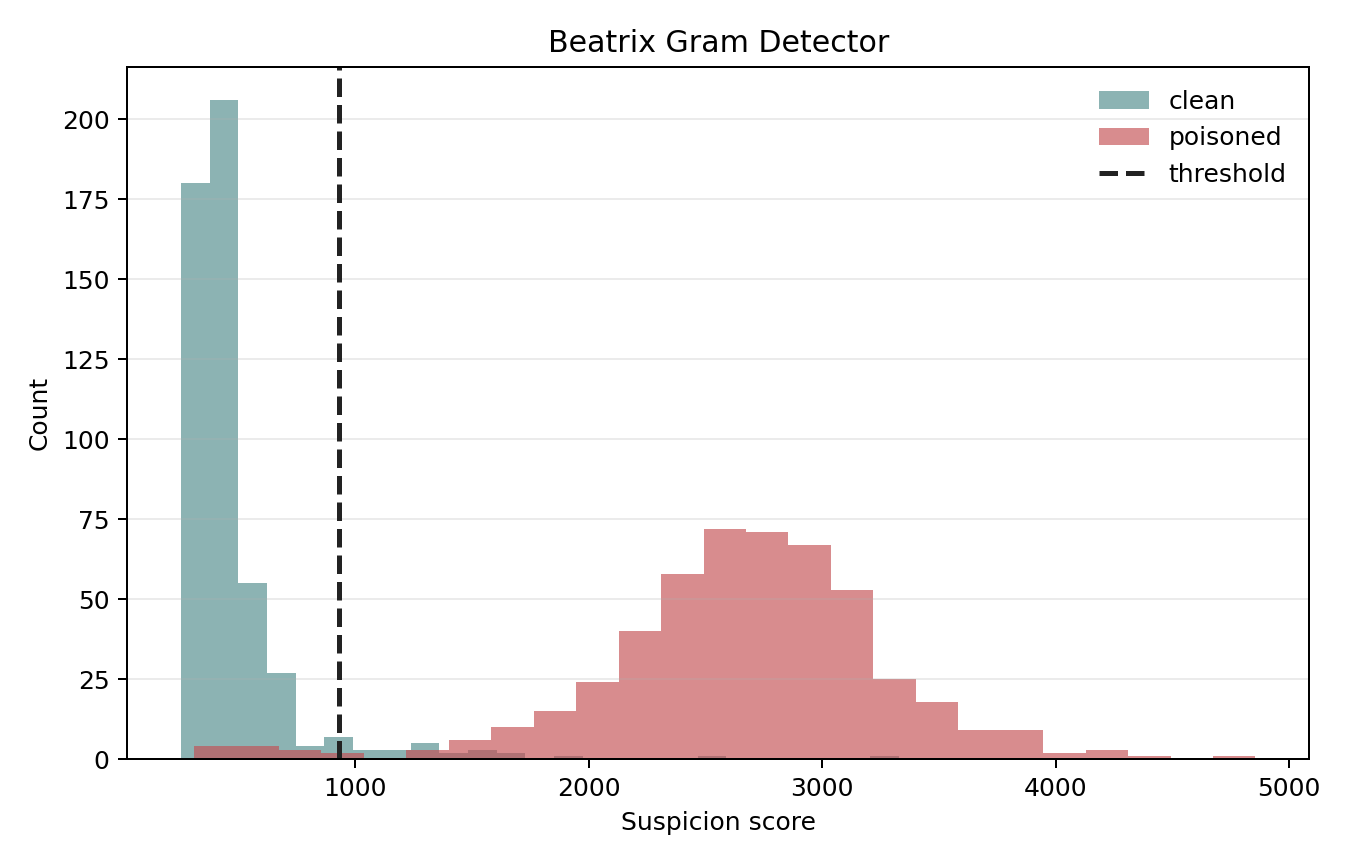
\includegraphics[width=0.28\textwidth]{figures/defense/beatrix_score_hist_blip2.png} &
        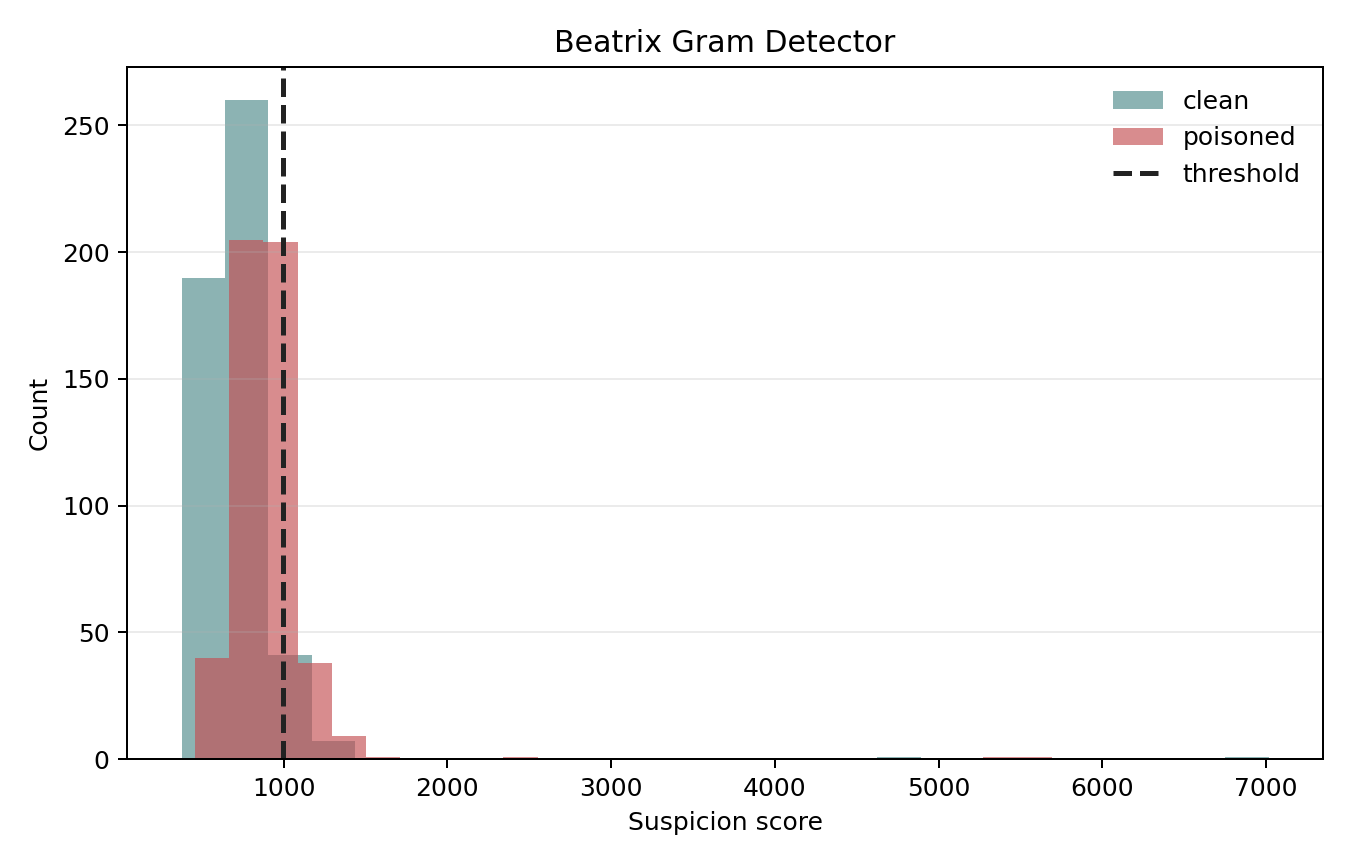
\includegraphics[width=0.28\textwidth]{figures/defense/beatrix_score_hist_instructBLIP.png} &
        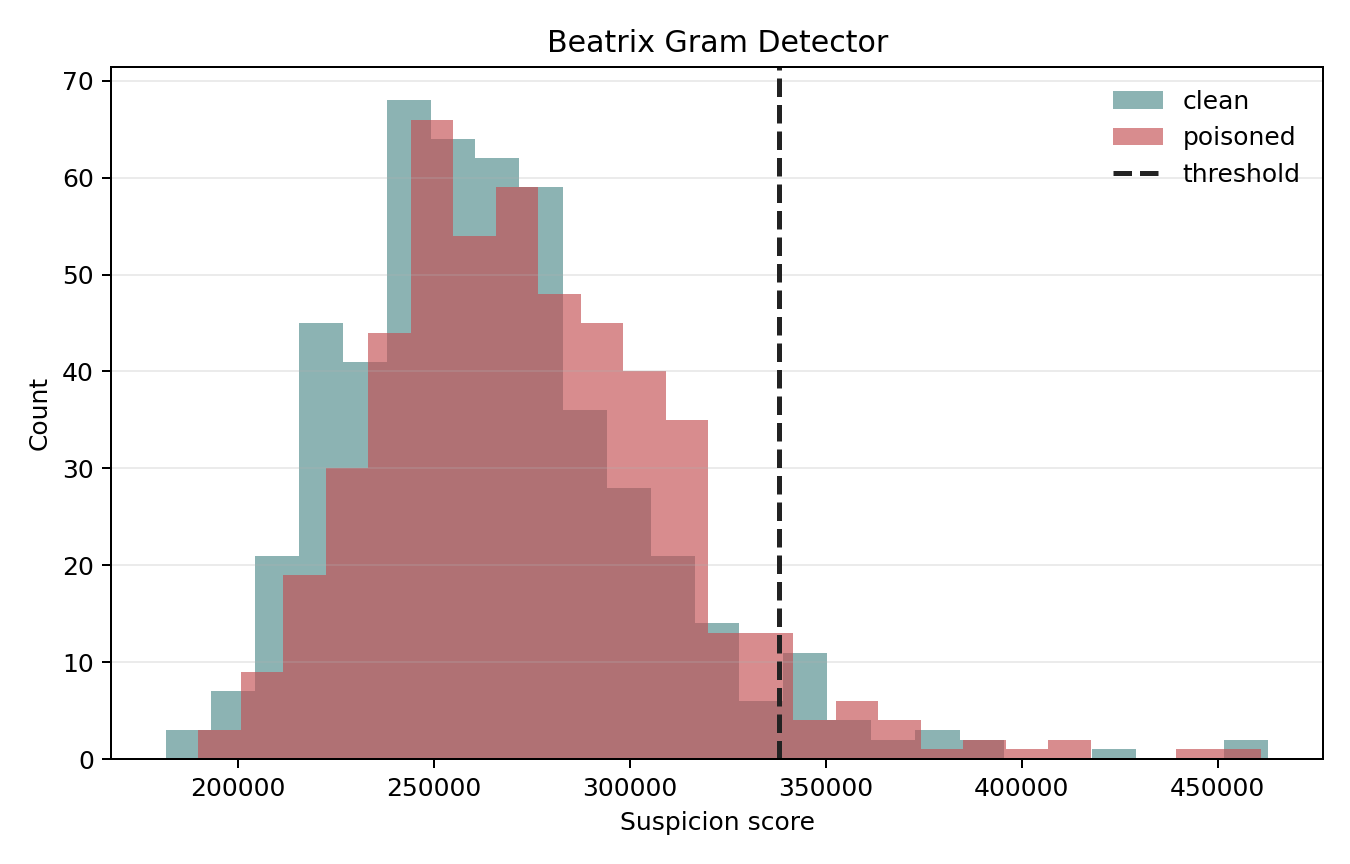
\includegraphics[width=0.28\textwidth]{figures/defense/beatrix_score_hist_llava.png} \\
        \textbf{\shortstack{Spectral\\Signatures}} &
        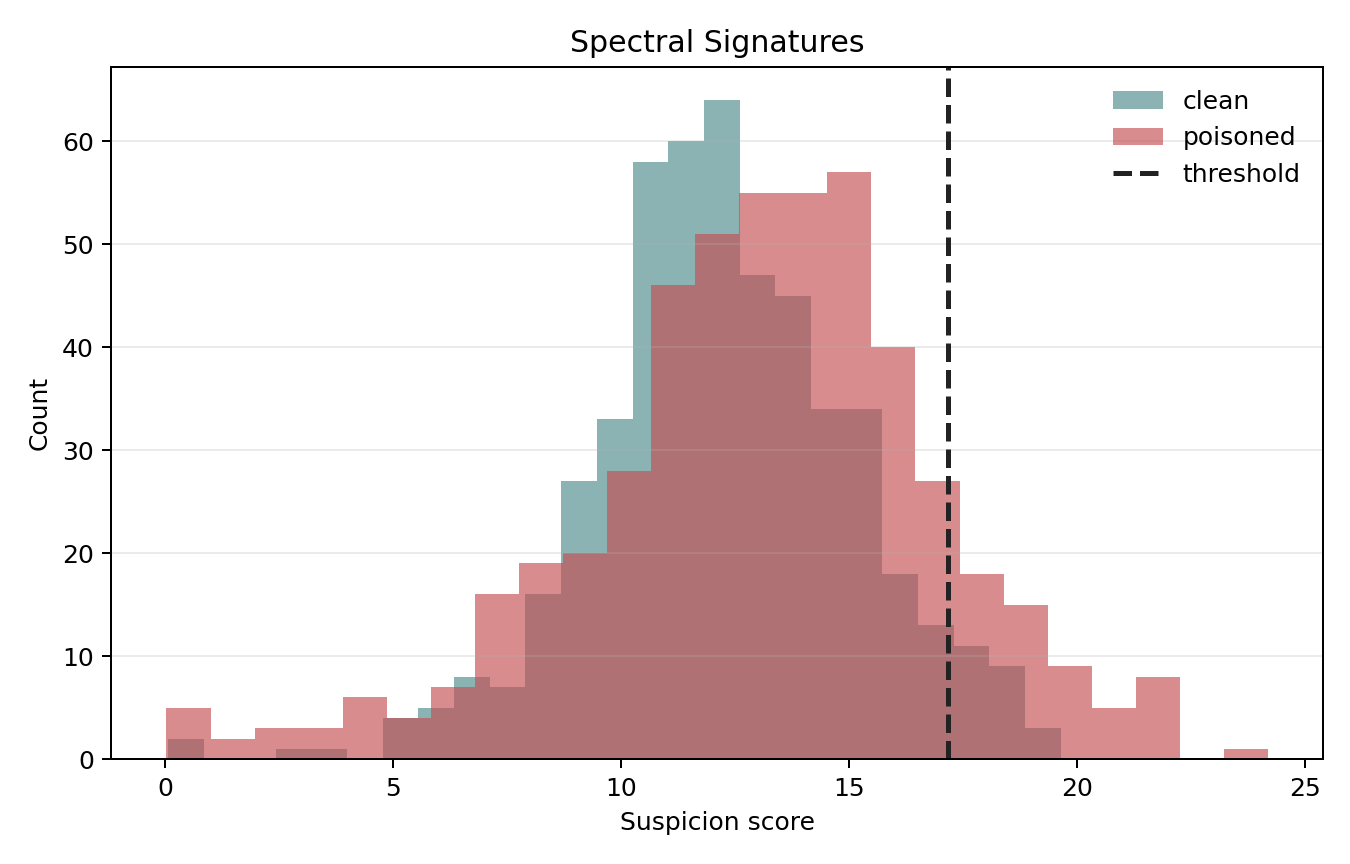
\includegraphics[width=0.28\textwidth]{figures/defense/spectral_score_hist_blip2.png} &
        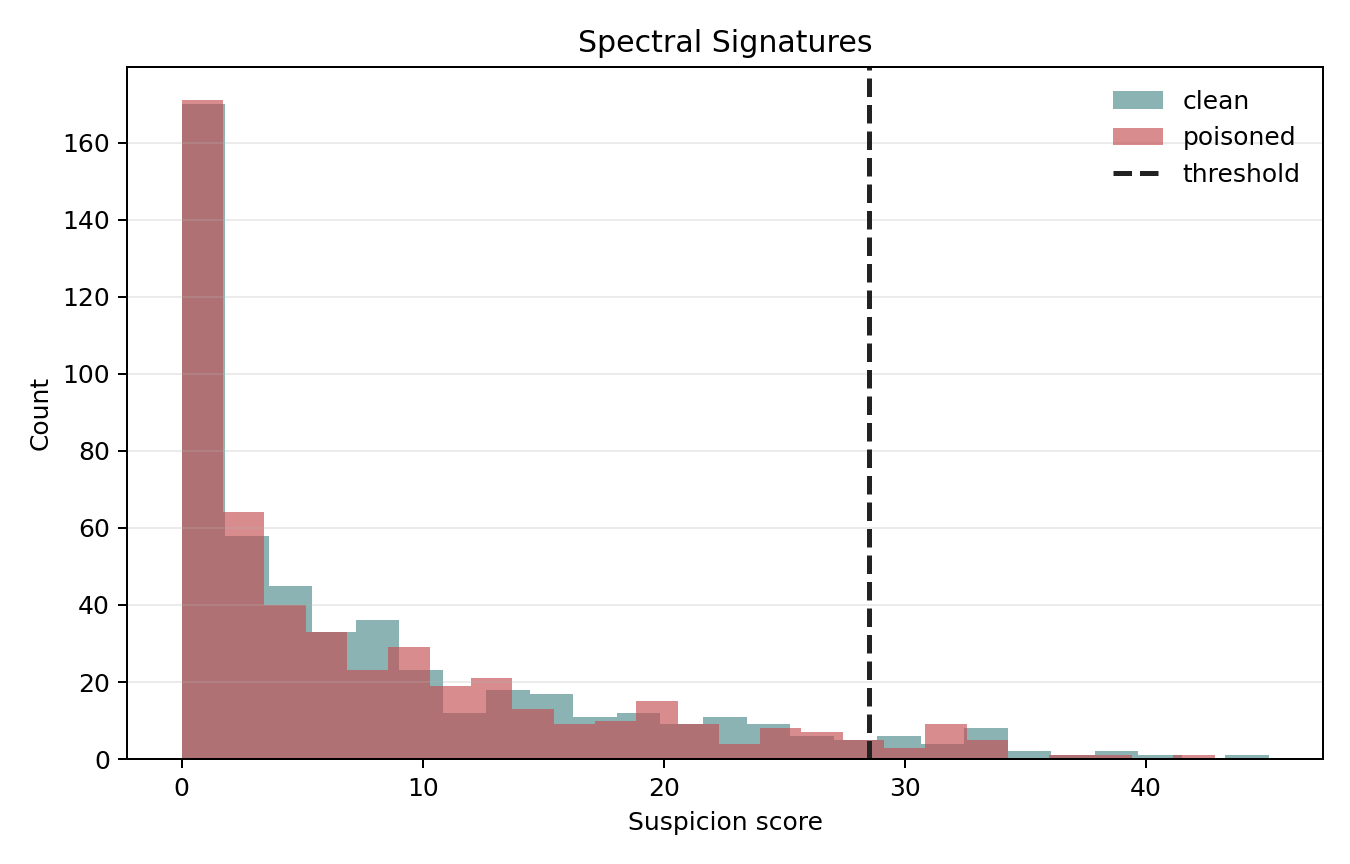
\includegraphics[width=0.28\textwidth]{figures/defense/spectral_score_hist_instructBLIP.png} &
        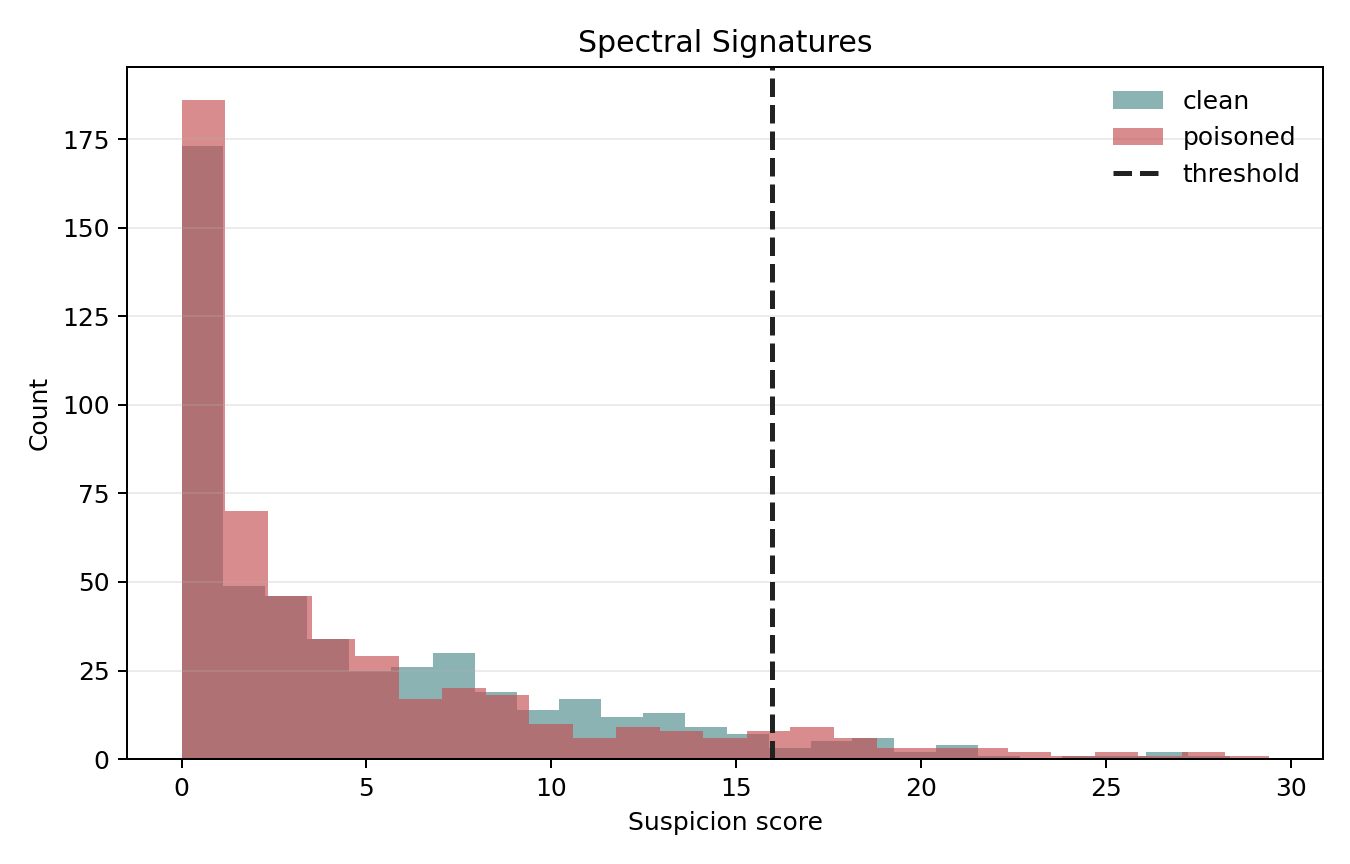
\includegraphics[width=0.28\textwidth]{figures/defense/spectral_score_hist_llava.png} \\
        \textbf{STRIP} &
        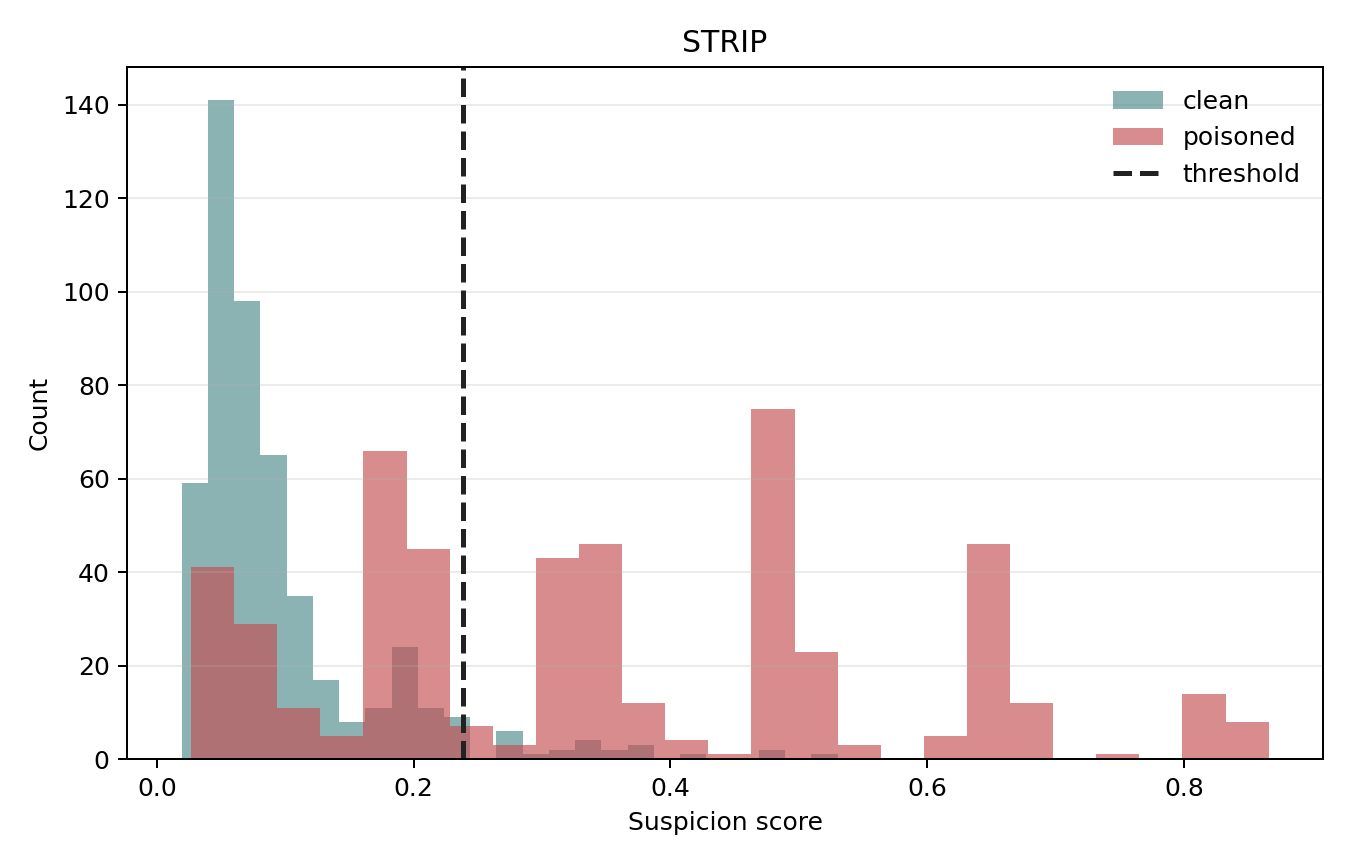
\includegraphics[width=0.28\textwidth]{figures/defense/strip_score_hist_blip2.png} &
        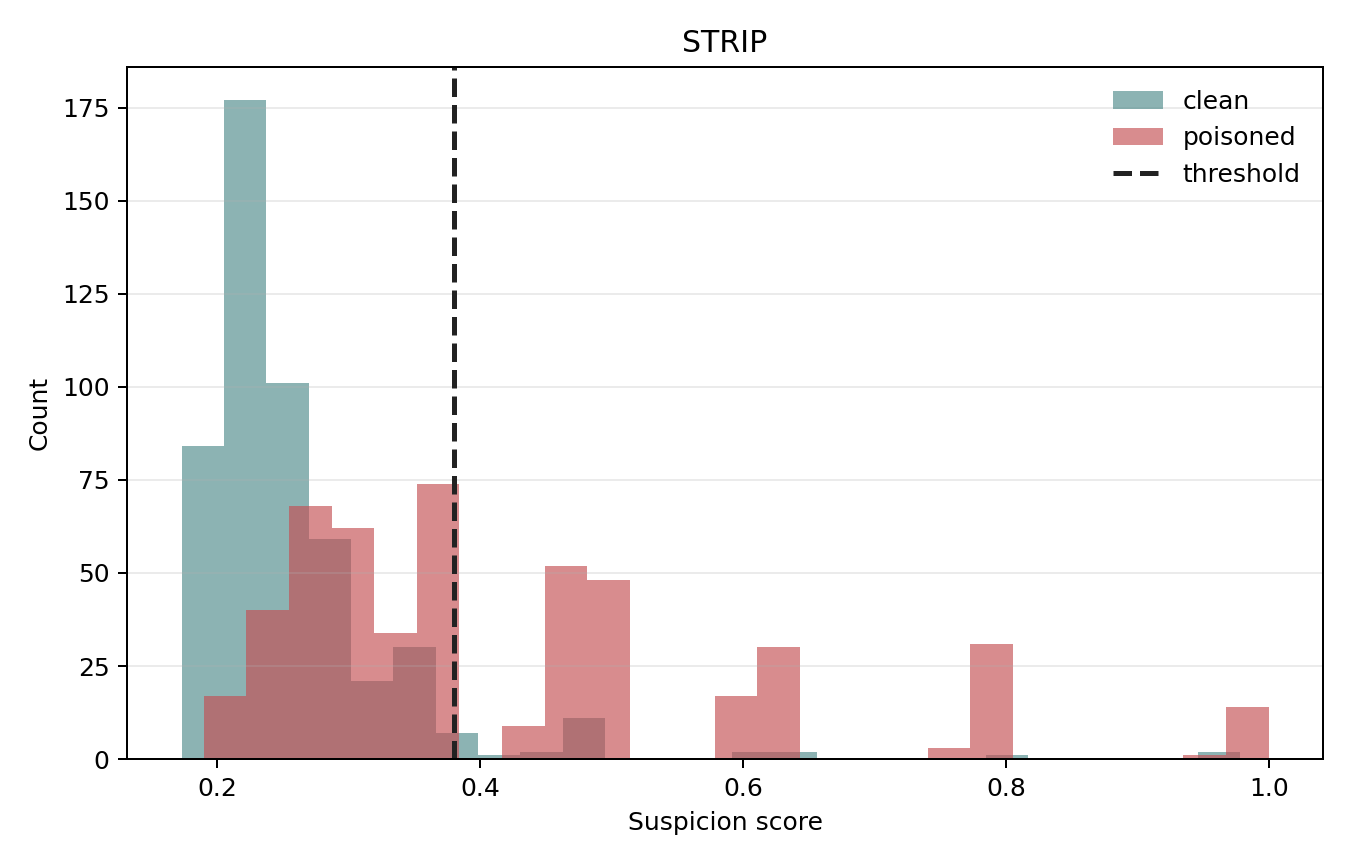
\includegraphics[width=0.28\textwidth]{figures/defense/strip_score_hist_instructBLIP.png} &
        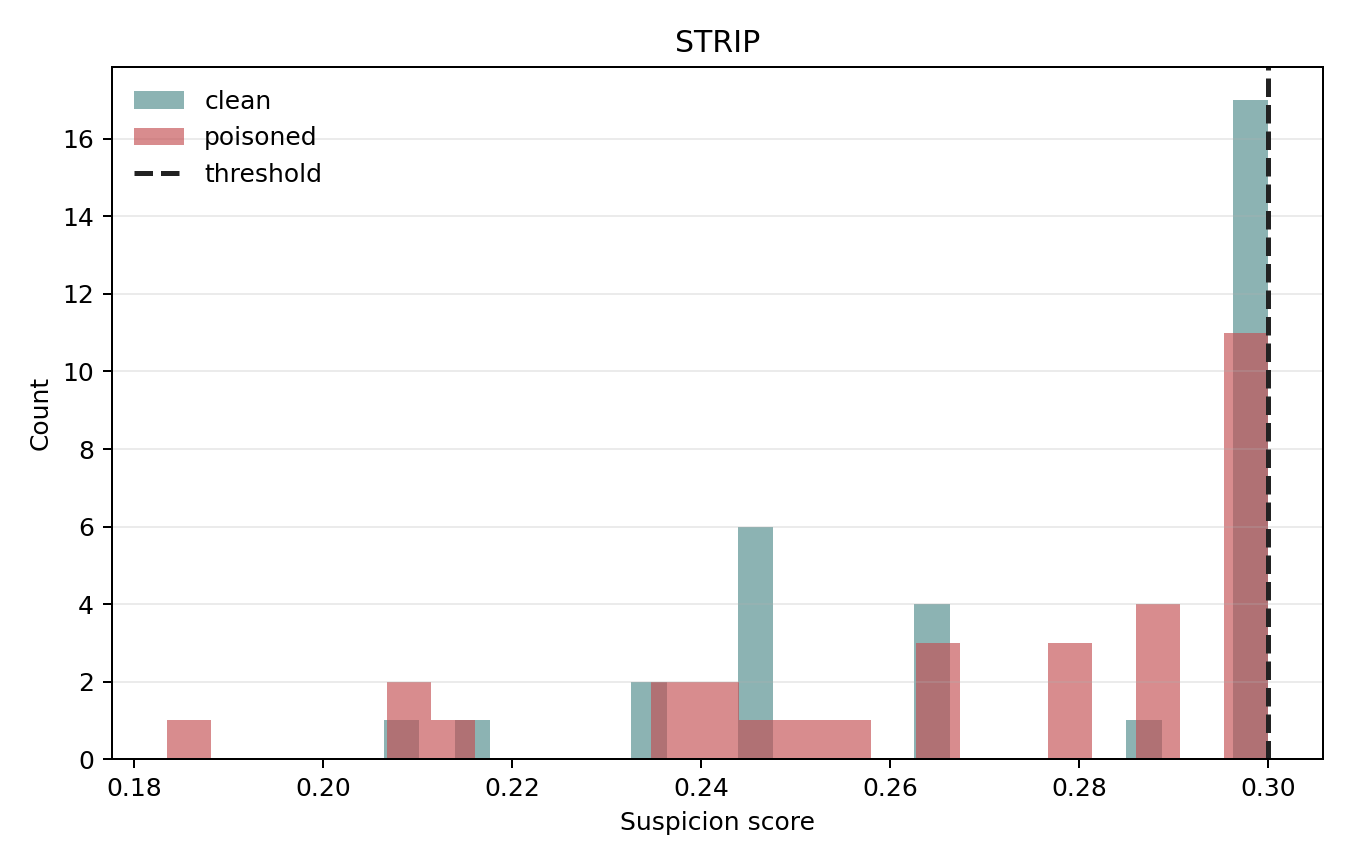
\includegraphics[width=0.28\textwidth]{figures/defense/strip_score_hist_llava.png} \\
    \end{tabular}
    \caption{Distribution of suspicion scores produced by three backdoor
    detectors on clean and frequency-triggered inputs across BLIP-2,
    InstructBLIP, and LLaVA. Rows correspond to Beatrix, Spectral
    Signatures, and STRIP, while columns correspond to the victim VLMs.
    The dashed vertical line in each histogram denotes the decision
    threshold. Strong overlap between the clean and poisoned
    distributions indicates difficulty in separating triggered samples
    from benign inputs.}
    \label{fig:defense_score_distributions}
\end{figure*}


\section{Ablation Study}
\label{sec:ablation}

We ablate two trigger-generation choices---the frequency mixing ratio and the selected frequency band---by varying each at inference with the model and evaluation protocol fixed. We report ASR for backdoor activation, PSNR and SSIM for visual similarity, and task-specific metrics for semantic utility.

\subsection{Effect of Frequency Mixing Ratio}
\label{subsec:ablation_ratio}
Within the selected mask, $r_s$ and $r_t=1-r_s$ control the clean-image and trigger-source contributions, respectively. We vary this ratio while keeping the Cartesian mask, unmasked-region ratio, trigger-source images, and other settings fixed.

% ratio mix
\begin{table*}[t]
\centering
\caption{Ablation study on the frequency mixing ratio. 
$r_s$ and $r_t$ denote the source- and trigger-frequency contributions inside the selected mask, respectively. 
Higher ASR indicates stronger backdoor activation, while higher PSNR and SSIM indicate better visual stealthiness.}
\label{tab:ratio_ablation}
\resizebox{\textwidth}{!}{
\begin{tabular}{c|cc|ccc|cc}
\hline
\multirow{2}{*}{\textbf{Model}} &
\multicolumn{2}{c|}{\textbf{Mixing Ratio}} &
\multicolumn{3}{c|}{\textbf{Attack / Utility}} &
\multicolumn{2}{c}{\textbf{Stealthiness}} \\
\cmidrule(lr){2-3}
\cmidrule(lr){4-6}
\cmidrule(lr){7-8}
& $\boldsymbol{r_s}$ & $\boldsymbol{r_t}$ & \textbf{ASR} $\uparrow$ & \textbf{METEOR} $\uparrow$ & \textbf{ROUGE-L} $\uparrow$ & \textbf{PSNR} $\uparrow$ & \textbf{SSIM} $\uparrow$ \\

\hline

\multirow{5}{*}{LLaVA}
& 0.95 & 0.05 & 0.204 & 0.506 & 0.441 & 32.91 & 0.933 \\
& 0.85 & 0.15 & 0.468 & 0.490 & 0.428 & 27.74 & 0.902 \\
& 0.75 & 0.25 & \textbf{0.552} & 0.483 & 0.4237 & 24.09 & 0.857 \\
& 0.65 & 0.35 & 0.540 & 0.488 & 0.429 & 21.43 & 0.804 \\
% & 0.55 & 0.45 & 0.516 & 0.4806 & 0.4289 & 19.38 & 0.7467 \\
\hline

\multirow{5}{*}{InstructBLIP}
& 0.95 & 0.05 & 0.316 & 0.558 & 0.561 & 32.96 & 0.935 \\
& 0.85 & 0.15 & 0.844 & 0.555 & 0.575 & 27.75 & 0.903 \\
& 0.75 & 0.25 & \textbf{0.940} & 0.549 & 0.568 & 24.09 & 0.858 \\
& 0.65 & 0.35 & 0.920 & 0.540 & 0.553 & 21.44 & 0.804 \\
% & 0.55 & 0.45 & 0.936 & 0.5409 & 0.5536 & 19.38 & 0.7469 \\
\hline

\multirow{5}{*}{BLIP-2}
& 0.95 & 0.05 & 0.244 & 0.465 & 0.558 & 32.96 & 0.935 \\
& 0.85 & 0.15 & 0.896 & 0.382 & 0.507 & 27.75 & 0.903 \\
& 0.75 & 0.25 & \textbf{0.992} & 0.372 & 0.511 & 24.09 & 0.858 \\
& 0.65 & 0.35 & \textbf{0.992} & 0.360 & 0.504 & 21.44 & 0.804 \\
% & 0.55 & 0.45 & \textbf{0.992} & 0.3656 & 0.4957 & 19.38 & 0.7469 \\
\hline

\end{tabular}
}
\end{table*}

% band ablation
\begin{table*}[t]
\centering
\caption{Frequency Band Ablation Study}
\label{tab:freq_band_ablation}
\begin{tabular}{ll ccc ccc ccc}
\toprule
\multirow{2}{*}{\textbf{Model}} & \multirow{2}{*}{\textbf{Band}} & \multirow{2}{*}{\textbf{ASR} $\uparrow$}  & \multirow{2}{*}{\textbf{PSNR}$\uparrow$} & \multirow{2}{*}{\textbf{SSIM} $\uparrow$} & \multicolumn{3}{c}{\textbf{Clean}} & \multicolumn{3}{c}{\textbf{Poisoned}} \\
\cmidrule(lr){6-8} \cmidrule(lr){9-11}
 & & & & & \textbf{BLEU-4} $\uparrow$ & \textbf{METEOR} $\uparrow$ & \textbf{ROUGE-L} $\uparrow$ & \textbf{BLEU-4} $\uparrow$ & \textbf{METEOR} $\uparrow$ & \textbf{ROUGE-L} $\uparrow$ \\
\midrule
\multirow{3}{*}{instructBLIP}
 & Low  & 0.504 & 29.227 & 0.957 & 0.129 & 0.557 & 0.552 & 0.121 & 0.555 & 0.565 \\
 & Mid  & 0.040 & 45.604 & 0.995 & 0.129 & 0.557 & 0.552 & 0.138 & 0.553 & 0.556 \\
 & High & 0.032 & 47.683 & 0.997 & 0.129 & 0.557 & 0.552 & 0.130 & 0.561 & 0.555 \\
\midrule
\multirow{3}{*}{LLaVA}
 & Low  & 0.545 & 29.227 & 0.957 & 0.079 & 0.517 & 0.442 & 0.066 & 0.506 & 0.440 \\
 & Mid  & 0.000 & 45.604 & 0.995 & 0.079 & 0.517 & 0.442 & 0.077 & 0.515 & 0.443 \\
 & High & 0.004 & 47.683 & 0.997 & 0.079 & 0.517 & 0.442 & 0.080 & 0.519 & 0.443 \\
\midrule
\multirow{3}{*}{BLIP2}
 & Low  & 0.560 & 29.227 & 0.957 & 0.135 & 0.482 & 0.567 & 0.077 & 0.429 & 0.537 \\
 & Mid  & 0.008 & 45.604 & 0.995 & 0.135 & 0.482 & 0.567 & 0.133 & 0.483 & 0.566 \\
 & High & 0.004 & 47.683 & 0.997 & 0.135 & 0.482 & 0.567 & 0.138 & 0.486 & 0.570 \\
\bottomrule
\end{tabular}
\end{table*}

Table~\ref{tab:ratio_ablation} shows the expected effectiveness--stealthiness trade-off: a small trigger contribution preserves image quality but activates the backdoor weakly, whereas increasing it to $15$--$25\%$ substantially improves ASR at the cost of lower PSNR and SSIM. The setting $r_s=0.75$, $r_t=0.25$ achieves the highest or joint-highest ASR on all three models and is the best choice when attack effectiveness is prioritized; $r_s=0.85$, $r_t=0.15$ provides a more stealth-oriented compromise. Increasing the trigger contribution beyond $25\%$ yields no further ASR gain and further degrades visual quality, suggesting that excessive trigger content acts mainly as image distortion. Thus, $r_s\in[0.75,0.85]$ provides the most useful operating range.

\subsection{Effect of Frequency Band Selection}
\label{subsec:ablation_band}

We further investigate the spectral sensitivity of the learned backdoor by restricting the trigger information to three representative frequency regions: low, middle, and high frequencies. During this experiment, the backdoored model and all other trigger-generation settings are kept fixed, while only the selected frequency region is varied. Therefore, this ablation evaluates which spectral components contribute most strongly to the activation of the already learned \textsc{FreqDoor} trigger. As shown in Table~\ref{tab:freq_band_ablation}, low-frequency components consistently produce the strongest backdoor activation across all evaluated VLMs, whereas the ASR drops sharply for the middle- and high-frequency settings. For instance, InstructBLIP achieves $50.4\%$ ASR in the low-frequency setting, compared with only $4.0\%$ and $3.2\%$ for the middle and high bands, respectively. A similar trend is observed for BLIP-2 and LLaVA. In contrast, higher-frequency modifications provide substantially better visual similarity, with PSNR increasing from $29.23$~dB in the low-frequency setting to $47.68$~dB in the high-frequency setting, while SSIM improves from $0.9568$ to $0.9973$. These results indicate that the learned backdoor is predominantly sensitive to lower-frequency components, while higher-frequency perturbations are more imperceptible but insufficient to reliably activate the trigger. Overall, the results reveal a clear trade-off between attack effectiveness and visual stealthiness across frequency bands.

\section{Limitations and Future Directions}
\label{sec:limitations}

Despite the effectiveness of \textsc{FreqDoor}, the present study has several limitations that define the scope of the proposed attack. First, we consider a white-box, training-time threat model in which the attacker has access to the model fine-tuning process and can inject poisoned samples during training. While this setting is relevant to compromised training pipelines or malicious model providers, it does not cover black-box or test-time attack scenarios. Extending \textsc{FreqDoor} to more restrictive attacker settings would therefore be an important direction for future work.

Second, the attack performance depends on the selected frequency configuration. As shown in the ablation study, the frequency band and mixing ratio directly influence both backdoor activation and perceptual similarity. Lower-frequency components generally provide a stronger trigger signal, whereas increasing the contribution of the trigger source can reduce image stealthiness. This reflects an inherent trade-off between attack effectiveness and imperceptibility. Future work could investigate adaptive or learnable strategies for automatically selecting the frequency bands and mixing parameters to achieve a better balance between these objectives.

\section{Conclusion}
In this work, we introduced \textsc{FreqDoor}, a frequency-domain backdoor attack for vision-language models that embeds visually imperceptible triggers by manipulating selected frequency components of the input image. We evaluated the attack across multiple VLM architectures and two representative vision-language tasks, including image captioning and visual question answering. The experimental results demonstrate that \textsc{FreqDoor} achieves high attack success while largely preserving clean-task performance and the semantic quality of generated outputs. Moreover, the proposed trigger provides improved visual stealthiness and shows robustness against several input-processing and backdoor-specific defenses. These findings highlight the vulnerability of current VLMs to frequency-domain backdoor manipulation and emphasize the need for more effective defense mechanisms for multimodal models.


% \begin{thebibliography}{1}
% \bibliographystyle{IEEEtran}
% \end{thebibliography}

% \newpage

\bibliographystyle{IEEEtran}
\bibliography{ref}


\section{Biography Section}
If you have an EPS/PDF photo (graphicx package needed), extra braces are
 needed around the contents of the optional argument to biography to prevent
 the LaTeX parser from getting confused when it sees the complicated
 $\backslash${\tt{includegraphics}} command within an optional argument. (You can create
 your own custom macro containing the $\backslash${\tt{includegraphics}} command to make things
 simpler here.)
 
\vspace{11pt}

\bf{If you include a photo:}\vspace{-33pt}
\begin{IEEEbiography}[{\includegraphics[width=1in,height=1.25in,clip,keepaspectratio]{fig1}}]{Michael Shell}
Use $\backslash${\tt{begin\{IEEEbiography\}}} and then for the 1st argument use $\backslash${\tt{includegraphics}} to declare and link the author photo.
Use the author name as the 3rd argument followed by the biography text.
\end{IEEEbiography}

\vspace{11pt}

\bf{If you will not include a photo:}\vspace{-33pt}
\begin{IEEEbiographynophoto}{John Doe}
Use $\backslash${\tt{begin\{IEEEbiographynophoto\}}} and the author name as the argument followed by the biography text.
\end{IEEEbiographynophoto}




\vfill

\end{document}
